%!TEX root = paper.tex
%
\documentclass[aps,twocolumn]{revtex4-1}
\pdfoutput=1

% amsmath package, useful for mathematical formulas
\usepackage{amsmath}
\setcounter{MaxMatrixCols}{50}
% amssymb package, useful for mathematical symbols
\usepackage{amssymb}

% graphicx package, useful for including eps and pdf graphics
% include graphics with the command \includegraphics
\usepackage{graphicx}

% cite package, to clean up citations in the main text. Do not remove.
% \usepackage{cite}

\usepackage{color}

% Use doublespacing - comment out for single spacing
%\usepackage{setspace}
%\doublespacing

% Text layout
% \topmargin 0.0cm
% \oddsidemargin 0.5cm
% \evensidemargin 0.5cm
% \textwidth 16cm
% \textheight 21cm

% Bold the 'Figure #' in the caption and separate it with a period
% Captions will be left justified
% \usepackage[labelfont=bf,labelsep=period,justification=raggedright]{caption}

% Leave date blank
\date{}

\pagestyle{myheadings}
%% ** EDIT HERE **

\usepackage{bussproofs}

% xy-pic for diagrams
\usepackage[all]{xy}
% subcaption
% \usepackage{subcaption}
% hyperref
% \usepackage[linkbordercolor={.67 .27 .27},citebordercolor={.09 .29 .54},urlbordercolor={.09 .29 .54}]{hyperref}
\usepackage{hyperref}
\hypersetup{colorlinks=true,
linkcolor=[rgb]{.67 .27 .27},
citecolor=[rgb]{.09 .29 .54},
urlcolor=[rgb]{.09 .29 .54}}
% \usepackage{natbib}
\usepackage[doipre={doi:}]{uri}

% color table cells http://goo.gl/ZmpJv
\usepackage[table]{xcolor}
% rotate text in table http://goo.gl/Lb4Zd
\usepackage{rotating}
% listings for code highlighting in appendix
\usepackage{listings}
\usepackage{setspace}
%!TEX root = ../plos_template.tex
% http://widerin.org/blog/syntax-highlighting-for-python-scripts-in-latex-documents
\definecolor{Code}{rgb}{0,0,0}
\definecolor{Decorators}{rgb}{0.5,0.5,0.5}
\definecolor{Numbers}{rgb}{0.5,0,0}
\definecolor{MatchingBrackets}{rgb}{0.25,0.5,0.5}
\definecolor{Keywords}{rgb}{.67, .27, .27}
\definecolor{self}{rgb}{0,0,0}
\definecolor{Strings}{rgb}{.09,.29,.54}
\definecolor{Comments}{rgb}{0,0.5,0}
\definecolor{Backquotes}{rgb}{0,0,0}
\definecolor{Classname}{rgb}{0,0,0}
\definecolor{FunctionName}{rgb}{0,0,0}
\definecolor{Operators}{rgb}{0,0,0}
\definecolor{Background}{rgb}{0.98,0.98,0.98}

\lstnewenvironment{python}[1][]{
\lstset{
numbers=left,
numberstyle=\footnotesize,
numbersep=1em,
xleftmargin=1em,
framextopmargin=2em,
framexbottommargin=2em,
showspaces=false,
showtabs=false,
showstringspaces=false,
frame=l,
tabsize=4,
% Basic
basicstyle=\ttfamily\small\setstretch{1},
%basicstyle=\ttfamily\footnotesize,frame=single,#1,
backgroundcolor=\color{Background},
language=Python,
% Comments
commentstyle=\color{Comments}\slshape,
% Strings
stringstyle=\color{Strings},
morecomment=[s][\color{Strings}]{"""}{"""},
morecomment=[s][\color{Strings}]{'''}{'''},
% keywords
morekeywords={import,from,class,def,for,while,if,is,in,elif,else,not,and,or,print,break,continue,return,True,False,None,access,as,,del,except,exec,finally,global,import,lambda,pass,print,raise,try,assert},
keywordstyle={\color{Keywords}\bfseries},
% additional keywords
morekeywords={[2]@invariant},
keywordstyle={[2]\color{Decorators}\slshape},
emph={self},
emphstyle={\color{self}\slshape},
%
}}{}

\usepackage{placeins}
\usepackage{longtable}
\usepackage{dot2texi}
\usepackage{tikz}
\usetikzlibrary{automata,shapes,arrows}
% todo notes see http://www.texample.net/tikz/examples/todo-notes/
\usepackage[colorinlistoftodos]{todonotes}
\usepackage{amsthm}
\usepackage{bibunits}

% define colors
\definecolor{DeepRed}{rgb}{.82,.14,.16}
\definecolor{DeepBlue}{rgb}{0,0.36,0.62}

% set depth for table of contents
% http://tex.stackexchange.com/a/17879/6784
% http://tex.stackexchange.com/a/11669/6784
\setcounter{tocdepth}{4}
\setcounter{secnumdepth}{0}

% copy of thebibliography from natbib
% to avoid indentation
% \makeatletter
% \def\@biblabel#1{}
% \renewenvironment{thebibliography}[1]{%
%  \bibfont\bibsection\parindent \z@\list
%    {\@biblabel{\arabic{NAT@ctr}}}{\@bibsetup{#1}%
%     \setcounter{NAT@ctr}{0}}%
%     \ifNAT@openbib
%       \renewcommand\newblock{\par}
%     \else
%       \renewcommand\newblock{\hskip .11em \@plus.33em \@minus.07em}%
%     \fi
%     \sloppy\clubpenalty4000\widowpenalty4000
%     \sfcode`\.=1000\relax
%     \let\citeN\cite \let\shortcite\cite
%     \let\citeasnoun\cite
%  }{\def\@noitemerr{%
%   \PackageWarning{natbib}
%      {Empty `thebibliography' environment}}%
%   \endlist\vskip-\lastskip}
% \makeatother

\makeatletter
\def\@biblabel#1{}
\renewenvironment{thebibliography}[1]{%
 \bibfont\bibsection\parindent \z@\list
   {\@biblabel{\arabic{NAT@ctr}}}{\@bibsetup{#1}%
    }%
    \ifNAT@openbib
      \renewcommand\newblock{\par}
    \else
      \renewcommand\newblock{\hskip .11em \@plus.33em \@minus.07em}%
    \fi
    \sloppy\clubpenalty4000\widowpenalty4000
    \sfcode`\.=1000\relax
    \let\citeN\cite \let\shortcite\cite
    \let\citeasnoun\cite
 }{\def\@noitemerr{%
  \PackageWarning{natbib}
     {Empty `thebibliography' environment}}%
  \endlist\vskip-\lastskip}
\makeatother


%% ** EDIT HERE **
%% PLEASE INCLUDE ALL MACROS BELOW

\newtheorem{theorem}{Theorem}[section]
\newtheorem{lemma}[theorem]{Lemma}

\theoremstyle{definition}
\newtheorem{definition}[theorem]{Definition}
\newtheorem{example}[theorem]{Example}
\newtheorem{xca}[theorem]{Exercise}

\theoremstyle{remark}
\newtheorem{remark}[theorem]{Remark}


% Set autoref text
% http://tex.stackexchange.com/a/36576/6784
\renewcommand*{\figureautorefname}{Fig.}
\renewcommand*{\equationautorefname}{Eq.}
\renewcommand*{\tableautorefname}{Table}
\renewcommand*{\sectionautorefname}{Sec.}
\renewcommand*{\subsectionautorefname}{Sec.}

\renewcommand{\refname}{References}

\newcommand{\beginsupplement}{%
        \setcounter{table}{0}
        \renewcommand{\thetable}{S\arabic{table}}%
        \setcounter{figure}{0}
        \renewcommand{\thefigure}{S\arabic{figure}}%
        \setcounter{equation}{0}
        \renewcommand{\theequation}{S\arabic{equation}}%
        \renewcommand*{\sectionautorefname}{Sec.}
     }

\def\tr{\mathrm{tr}}
\def\Path{\mathrm{Path}}
\def\hier{\mathbf{Hier}}
\def\Vertex{\mathrm{Vertex}}
\def\adj{\mathrm{adj}}
\def\wprod{\mathbf{wp}}
\def\length{\mathbf{len}}
\def\connectivity{d}
\def\reffigexamplesystemmodules{\ref{fig:modsccsym}A}
\def\reffigscc{\ref{fig:modsccsym}B}
\def\reffighiertransformations{\ref{fig:modsccsym}C}
\def\reffigrobustconnect{\ref{fig:combined}A}
\def\reffigrobusthierarchy{\ref{fig:combined}B}
\def\reffigconnectcycle3D3x3{\ref{fig:combined}C}
\def\reffigconnectdist3D3x3{\ref{fig:combined}D}
\def\refsupp{Supplementary Material}
%% END MACROS SECTION


\begin{document}

% Add Figure, Table prefixes to references
% http://tex.stackexchange.com/a/6063/6784
\let\ref\autoref

\title{Ensemble Stability of Biological Networks}

\pagenumbering{arabic}

% Title must be 150 characters or less
\begin{center}
{\Large
\textbf{Hierarchical Network Structure Promotes Dynamical Robustness}
}
% Insert Author names, affiliations and corresponding author email.
\\[.5cm]
Aviv Bergman$^{1,2,3,4}$,
Raymond S. Puzio$^{1}$,
Cameron Smith$^{1}$,
\\[.5cm]
$^1$Department of Systems and Computational Biology,\\
$^2$Dominick P. Purpura Department of Neuroscience,\\
$^3$Department of Pathology, Albert Einstein College of Medicine,\\
1301 Morris Park Ave, Bronx, NY 10461, USA\\
$^4$Santa Fe Institute, 1399 Hyde Park Road, Santa Fe, NM 87501, USA
\\[.5cm]
% $\ast$To whom correspondence should be addressed; E-mail: aviv@einstein.yu.edu.
\end{center}

{\begin{quote} \bf
%!TEX root = ../paper.tex
The analysis of dynamical systems that attempts to model chemical reaction, gene-regulatory, population, and ecosystem networks all rely on models having interacting components. When the details of these interactions are unknown for systems of interest, one effective approach is to study the dynamical properties of an ensemble of models determined by constraints that can be considered to apply to all such systems. Here we analyze the stability and robustness of a large class of dynamical systems. In particular, we precisely determine the probability distribution of robustness over system connectivity, which has significant implications from the study of metabolic to gene-regulatory to ecosystem network dynamics, for systems with two and three interacting components. We show that robustness is classified by the number of links between strongly connected components of the graph representing the underlying system connectivity leading to the conclusion that the most robust systems are also the most hierarchical. We also demonstrate that permutation of strongly connected components is a fundamental symmetry of dynamical robustness. This results in the classification of the dynamical robustness of biological networks based upon a purely topological property.

\end{quote}}

% \section{Todo}
\listoftodos
\tableofcontents

\section{Introduction}

The traditional approach taken in the study of chemical reaction, gene-regulatory, population, and ecosystem networks is to consider a particular example, derive a system of differential equations to model that example, try to fit the model to data and adjust the modeling assumptions along with parameter values until a good fit is achieved \cite{Meyer2014}. Recent work has demonstrated that as a result of sloppiness in the dependence of qualitative dynamic phenomena on the geometry of parameter space that this approach allows for a large variety of models to fit the data \cite{Brown2003,Gutenkunst2007,Daniels2008a,Machta2013,Hines2014,Prabakaran2014,Tonsing2014}. In the face of uncertainty about the structure of such biological networks, to model the components under consideration as randomly interlinked becomes a reasonable approximation. This approach enables one to gain insight into what dynamical phenomena are possible to observe within a given class of dynamical systems, which is necessary to understand in order to determine whether or not a particular dynamical phenomenon should be regarded as unique or generic in the development and investigation of models applied to particular systems \cite{Gunawardena2013,Gunawardena2014}.

Indeed, investigating generic properties of a large class of dynamical systems was the approach taken by May in models of ecosystem dynamics \cite{Gardner1970,May1972}. The class of dynamical systems studied by May is so general that to restrict its applicability to ecosystem dynamics is certainly not necessary and perhaps even inefficient with respect to the goal of understanding how biological networks operate across the various relevant levels of organization. For example, the study of chemical reaction, population, and gene-regulatory networks all utilize essentially equivalent mathematical structure as that discussed by May in the context of ecosystem dynamics \cite{RossCr2003,Alon2006,Palsson2006,HamidBolouri2008,Palsson2011a,Voit2012,Sauro2012}. Developing unified mathematical descriptions of all of these is one of the paramount goals of systems biology. This incredibly generic applicability of gaining a better understanding of the class of models investigated by May demonstrates the unequivocal value of deeper investigation.  However, work attempting to continue the development of the so-called May-Wigner stability theorem revealed that May's conjectured stability criterion was not as easy to demonstrate as was initially believed \cite{Cohen1984,May1972a,Radius2014}.

Here we build on work aimed at investigating the stability of randomly connected dynamical systems to structural perturbations. We precisely compute the probability of stability as a distribution over system connectivity for all systems containing two or three interacting components. We then proceed to determine the probability of \emph{robustness} or \emph{structural stability} which is the distribution of stability to perturbation in the system structure for systems which are determined to be stable \cite{Smale1967}. This quantity is of interest at all scales of the biological hierarchy, and has been previously addressed in the study of the robustness of gene-regulatory networks \cite{WADDINGTON1942a,VanNimwegen1999,Siegal2002,Ciliberti2007b,Ciliberti2007,Wagner2013}. We find that stability to structural perturbations of this class of dynamical systems is correlated with connectivity, number of cycles, and the number of links between strongly connected components of the underlying interdependency graph. The latter derives from the fact that the permutation of strongly connected components is a symmetry of system robustness. This work clarifies a thread of research that is extremely important for the continuing development of systems biology.

\section{Dynamical systems on biological networks}
In the construction of a class of potential models for biological systems at any level of the biological hierarchy from metabolic to ecosystem-level networks, it is common to first attempt to define a collection of observable phenomena of interest and determine a domain (such as binary numbers, integers, or real numbers) in which each observable can be quantified. Next, it is necessary to establish the interdependencies among system components. The specific manner in which the components depend upon one another must be clarified, which is often done by determining a particular system of mathematical functions that represents a hypothesis about how the quantified observables evolve in time. To the degree to which there is uncertainty about the interactions among system components, parameters are introduced to broaden the class of models under consideration. Finally, whatever model class remains may be compared to empirical observations to determine how capable the model is of representing the phenomena of interest.

For the case of continuous deterministic observables, the above process can be made more precise by associating a manifold $M_i$ to each observable, a directed graph, $G$, to the interdependencies, and a vector field $V \in \Gamma T(\prod_i M_i)$ over the space determined by taking the product of the manifolds associated to the collection of observables, satisfying these interdependencies for each observable  \cite{Deville}. For example, if we have two observables $\{x_1,x_2\}$ where the domains in which they are quantified are given by manifolds $\{M_1,M_2\}$ such that $x_1 \in M_1 \equiv \mathbb{R}^1$ and $x_2 \in M_2 \equiv \mathbb{R}^1$, a directed graph $G_X$ describing the dependencies between these observables and vector field $V$ with components $\{F_1,F_2\}$ defined on $M_1 \otimes M_2 \equiv \mathbb{R}^2$ satisfying the dependencies determined by $G_X$. If the system under consideration has the graph given in \ref{fig:examplesystemmodules}A
% \begin{center}
% %!TEX root = ../paper.tex
\begin{tikzpicture}[
every state/.style={draw=red!50,very thick,fill=red!20}]
\begin{dot2tex}[styleonly,codeonly,neato,mathmode]
digraph G {
d2ttikzedgelabels = true;
node [style="state"];
edge [lblstyle="auto",topath="bend left",style="line width=1.5pt"];
x_1 -> x_2;
x_2 -> x_1;
x_2 -> x_2 [topath="loop above"];
}
\end{dot2tex}
\end{tikzpicture}

% \end{center}
with adjacency matrix
$$
\adj(G_X) = \begin{pmatrix}
0 & 1 \\
1 & 1
\end{pmatrix}
$$
having connectivity $\connectivity$ equal to the number of edges of the graph, in this case $\connectivity = 3$. For a general system the directed graph $G_X$ that describes the manner in which each of the variables depends upon one another is given by the adjacency matrix $\adj(G_X)$ where
 \begin{displaymath}
   \adj(G_X)_{ij} = \left\{
     \begin{array}{ll}
       1, & F_i \hbox{ depends on } x_j\\
       0, & F_i \hbox{ does not depend on } x_j
     \end{array}.
   \right.
\end{displaymath} For the system $X = \{G_X, M_X, F_X\}$, where $M_X \equiv \{M_1,M_2\}$ and $F_X \equiv \{F_1,F_2\}$ such that $F_1$ is constrained to be a function of $x_2$ and $F_2$ is a function of both $x_1$ and $x_2$ yielding the flow equations
\begin{align*}
\frac{dx_1}{dt} & = F_1(x_2)\\
\frac{dx_2}{dt} & = F_2(x_1,x_2)
\end{align*}

In the more general case of a system with $n$ components we would have an $n$-dimensional vector of observables
$$
x(t) = (x_1(t), \ldots x_n(t)) = \vec{x}(t)
$$
whose components are solutions to the arbitrary first order system
$$
\frac{dx_i(t)}{dt} = F_i(\vec{x}(t)), \; (i=1,\ldots,n)
$$
where $F_i$ represent, potentially nonlinear, functions of the given vector of state variables.

\todo{Generalize to open systems and say how we combine them.}

In order to accommodate the possibility of uncertainty in our modelling,
we will generalize our notion of a system on a network to that of a
system with random parameters.  Again, this will involve three
steps. First, we provide a measure space $S, \mathcal{B}(S)$ which represents the
values over which our parameters can vary. Next, instead of a single
vector field, we consider a family of vector fields parameterized by
this space. That is to say, we introduce a mapping $V \colon S \to \Gamma T(\prod_i M_m)$.
(Here $\Gamma$ denotes the space of sections of the tangent bundle.)
As before, for each point $p \in S$, the vector field $V(p)$ must be consistent with
the system graph. Finally, we select a probability measure $\mu \colon
\mathcal{B}(S) \to [0,1]$ which represents our understanding of which values of the parameters
are likely. In accord with Bayesian statistics, we might revise this
distribution as data comes in or use it to estimate parameters and error
bars from experimental results.

Having done this, we are now in a position to do a probabilistic analysis
of our system and its properties.  Given some quantity $q$ characterizing
our system, this quantity becomes a random variable which may be discrete or
continuous depending on the quantity under consideration.  For example, if
the quantity is the time it takes for a particle to travel between two points,
we have a real-valued random variable; if the quantity is the number of fixed
points, we have an integer-valued random variable; and if the quantity is
whether or not the system posesses a limit cycle, we have a binary random
variable.

Another question one can ask is that of robustness, which measures the
probability that, if some property holds for a set of parameters, it will
continue to hold if we make a random perturbation about those parameter values.
To define robustness, we will introduce, in addition to the probability
distribution $\mu$ described above, a family of probability distributions
$\mu' \colon S \times \mathcal{B}(S) \to [0,1]$.  Then, given a binary random
variable $q$, we define its robustness as the following conditional proability:
\begin{align}\label{eq:robustness}
  R (q) =
  \frac{\int_S d\mu(x) \int_S d\mu'(x,y) \mathbf{1}_q(x) \mathbf{1}_q(y)}
  {\int_S d\mu(x) \mathbf{1}_q(x)}
\end{align}

\section{Stability analysis of biological networks}
Linearization of the $F_i$ about any fixed point $\vec{x}^0$ such that $F_i(\vec{x}^0)=0$ leads to the system
\begin{equation}\label{eq:lineardynsys}
\frac{d\vec{y}(t)}{dt} = A \vec{y}(t),
\end{equation}
where $\vec{y} = \vec{x} - \vec{x}^0$ and the $n \times n$-matrix $A$ has components
$$
a_{ij} = \left. \frac{\partial F_i}{\partial x_j} \right|_{\vec{x} = \vec{x}^0}.
$$
To each dynamical system having Jacobian matrix $A$ at some fixed point $\vec{x}^0$ we can associate a directed graph $G_A$ given by an adjacency matrix $\adj(G_A)$ where
 \begin{displaymath}
   \adj(G_A)_{ij} = \left\{
     \begin{array}{lr}
       1, & a_{ij} \neq 0\\
       0, & a_{ij} = 0
     \end{array}
   \right.
\end{displaymath}
The graphs $G_X$ and $G_A$ are equivalent because the condition $F_i$ independent of $x_j$ definitive of $\adj(G_X)$ corresponds precisely to $\frac{\partial F_i}{\partial x_j}=0$.

The spectral abscissa of the matrix $A$ is defined as
$$
\eta(A) = \max_i \{\Re(\lambda_i)\}
$$
where $\lambda_i$ are the eigenvalues of $A$. The system defined by $F_i$ and $\vec{x}^0$ is dynamically stable if the spectral abscissa of $A$ is less than zero, equivalently, $\eta(A) < 0$. This is because the general solution to \ref{eq:lineardynsys} is
$$
y_i(t) = \sum_j b_{ij} e^{\lambda_j t}, \; (i=1,\ldots,n)
$$
for some matrix $B=(b_{ij})$ and thus all $\vec{y} = \vec{x} - \vec{x}^0$ decay to zero when all $\lambda_i < 0$.

To determine whether a randomly selected dynamical system evaluated at a random critical point, given by a matrix such as $A$, is stable, it is sufficient to check the above condition. Integrating over the region of the parameter space defining $A$ enables the determination of the probability of stability to perturbations in state $\vec{x}$ over an ensemble of dynamical systems.

% Another form of stability, referred to as structural stability \cite{Smale1967}, requires the determination of whether or not a given dynamical system that is determined to be stable remains stable under a perturbation to one of its defining parameters. This can be formalized as the conditional probability distribution
% $$
% P(A' \, \textrm{stable}\, \big| \, A \, \textrm{stable})
% $$
% where $A'$ represents a matrix derived from some perturbation applied to the matrix $A$ given above. In the simple case where $A \in \mathbb{R}^{n \times n}$ the perturbation which involves sampling uniformly over the $a_{ij}$ defining $A$ the value of a particular $a_{ij}$ from a given probability distribution.
Suppose that $M$ is an $n \times n$ matrix with real coefficients and connectivity $\connectivity$. We will consider the case in which each of the parameters defining the matrix is sampled from the uniform distribution $\mathcal{U}(-1,1)$ so that the parameter space corresponds to the $\connectivity$-dimensional hypercube, $H^\connectivity$, of edge length $r=2$, centered about the origin, and having volume $r^\connectivity$.  We want to know the probability that, if we resample the elements $k_1, k_2, \ldots k_m$ of this matrix, the resulting matrix will correspond to a stable matrix.  This is a special case of \ref{eq:robustness}:
\begin{equation}\label{eq:condprobgen}
 R (\mathrm{stab}, k_1, \ldots k_m) =
  \frac{\int_{H^\connectivity} dx_1 \cdots dx_d \int_{H^m} {dx'}_{k_1} \cdots {dx'}_{k_m}\,
    \mathbf{1}_{stab} \mathbf{1}_{stab'}}
  {\int_{H^\connectivity} dx_1 \cdots dx_d  \, \mathbf{1}_{stab}(x_1 \cdots x_d)}
\end{equation}
where we made the abbreviations
\begin{align*}
\mathbf{1}_{stab} &= \mathbf{1}_{stab}(x_1 \cdots x_{k_1} \cdots x_{k_m} \cdots x_\connectivity) \\
\mathbf{1}_{stab'} &= \mathbf{1}_{stab'}(x_1 \cdots {x'}_{k_1} \cdots {x'}_{k_m}  \cdots x_d)
\end{align*}
i.e. $\mathbf{1}_{stab'}$ corresponds to replacing $x_{k_1}, \ldots x_{k_m}$ with their primed counterparts.

While one can resample a fixed subset of the links, more typically we will be randomly selecting which links to resample with a uniform distribution on the links.  The result of this operation corresponds to averaging our quantity over subsets of links:
\begin{equation}
R (\hbox{avg stab}, m) =
\frac{1}{\binom{\connectivity}{m}}
\sum_{\{k_1, k_2, \ldots k_m\} \subset \{1, 2,, \ldots \connectivity\}}
R (\mathrm{stab}, k_1, \ldots k_m)
\end{equation}

In order to evaluate these integrals, one needs to describe the stable region.
The theory of how to do so in terms of conditions on the coefficients of the
characteristic polynomials was developed by various mathematicians during the
second half of the nineteenth century and is summarized in chapter XV of
\cite{Gantmacher1959}.  We now summarize some of these results which are
relevant to our calculations.

\todo{Finish writing these criteria with reference to Gantmacher}
Define the characteristic polynomial as $\chi(M)(z) = \det(zI - M)$.
Denote the coefficients of $\chi(M)$ as $s_j$ and its roots as $r_j$,
writing $p(x) = x^n + \sum_{k=1}^n s_k x^{n-k} = \prod_{k=1}^n (x-r_k)$.
Then, since the roots of $\chi$ are the eigenvalues of $M$, asking that
$M$ be stable is equivalent to asking that the roots of $\chi$ all have
negative real part.  Hence, let us call a polynomial stable if all its
roots have negative real part.  We will formulate conditions for this to
happen in terms of the coefficients of $\chi$ \cite{Gantmacher1959}.

\begin{lemma}
If $M$ is stable, then $s_i > 0$ for all $i$ between $1$ and $n$.
\end{lemma}
\begin{lemma}
If a point lies on the boundary of the set of stable polynomials, then
either $s_n = 0$ and $\Delta = 0$.
\end{lemma}
\begin{lemma}
If $n < 6$, then a polynomial $p$ is stable if and only
if $\Delta > 0$ and $s_1 > 0$ for all $i$.
\end{lemma}

\section{Network hierarchy and strongly connected components}

A graph can be decomposed into a natural collection of \emph{modules} called strongly connected components. A strongly connected component of a graph is a maximal subset of vertices where each vertex within the subset can be reached from any other \cite{Cormen2009}. The strongly connected components of some examples of three component systems are outlined in \ref{fig:scc} along with their adjacency matrices and hierarchy diagrams (to be defined below).
\todo{add hierarchy diagrams to \ref{fig:scc}}

The decomposition of a digraph into strongly connected components corresponds to a block triangular decomposition of its adjacency matrix.  Say that the graph $G$ has strongly connected components $C_1, C_2, \ldots C_n$, which have been labelled in such a way that there are no links from vertices in component $C_i$ to component $C_j$ when $i < j$.  Label the vertices in such a way that $v_1, \ldots, v_{n_1}$ belong to $C_1$, $v_{n_1 + 1}, \ldots, v_{n_2}$ belong to $C_2$, etc.  Then, if we choose basis vectors corresponding to this labelling of the vertices, we will have $a_{ij} = 0$ whenever $i$ and $j$ correspond to different components and $i > j$.  This condition is equivalent to stating that the matrix is block triangular with blocks of size $n_1, n_2, \ldots$.

Corresponding to this decomposition we can construct a directed acyclic graph $\hier (G)$.  Each node of $\hier (G)$ corresponds to a strongly connected component of $G$. There is an edge from the node corresponding to component $C$ to the node corresponding to component $C'$ if and only if there exists a link from some vertex in $C$ to some vertex in $C'$ in $G$.  Because of the maximality of strongly connected components, $\hier (G)$ is acyclic.

One can also perform this construction in the oppsite direction.  Start with a directed acyclic graph $A$.  To each node $n$ of $A$ associate
a strongly connected graph $C_n$.  To each link $(i,j)$ of $A$ associate a non-empty subset of $\Vertex(C_i) \times \Vertex(C_j)$.  The result will be a graph $G$ such that $\hier(G) = A$ and furthermore, every graph $G$ such that $\hier(G) = A$ can be obtained in this manner.
\todo{explain how robustness in \ref{eq:robustness} is symmetric under permutations of the SCCs in $G$ or equivalently of the nodes of $\hier{G}$.}

\todo{add panel to \ref{fig:scc} showing that many graphs get mapped to the same SCC DAG}

\todo{add definition of graph edit distance to the most hierarchical network and define this as our measure of hierarchy}

\section{Stability and robustness analysis of particular system ensembles}
For systems having two components, we can analytically compute the probability of stability and robustness from \ref{eq:condprobgen}. For those having three components, we can estimate these same quantities using Monte Carlo simulations. Systems of larger size can be analyzed using the symmetry properties of robustness extracted from this analysis. For two-component systems having $2 \times 2$ Jacobian matrices, the aforementioned stability criteria result in the conditions $T < 0$ and $D >
0$ where $T$ and $D$ denote the trace and the determinant. Suppose we have a stable matrix
$$
\begin{pmatrix}
a & b \\
d & c
\end{pmatrix}
$$
where $a + c < 0$ and $ac > bd$.  For the case in which $x_1=a,\,x_2=b,\,x_3=c,\,x_4=d$ we need to compute what corresponds to $R(\mathrm{stab},k)$ where $k=1 \ldots 4$. By symmetry, there are two cases to consider; resampling $a$ is equivalent to resampling $c$ and resampling $b$ is equivalent to resampling $d$ so we only need to explicitly compute $R(\mathrm{stab},1)$ and $R(\mathrm{stab},2)$. Suppose that we resample $b$ to compute $R(\mathrm{stab},2)$.
% \begin{strip}
% \begin{align}\label{eq:condprob}
% P\left(\begin{pmatrix}
% a & b' \\
% d & c
% \end{pmatrix} \textrm{stable } \bigg| \begin{pmatrix}
% a & b \\
% d & c
% \end{pmatrix} \textrm{stable } \right)
% & = \frac{P\left(\begin{pmatrix}
% a & b \\
% d & c
% \end{pmatrix} \textrm{stable and } \begin{pmatrix}
% a & b' \\
% d & c
% \end{pmatrix} \textrm{stable } \right)}{P\left(\begin{pmatrix}
% a & b \\
% d & c
% \end{pmatrix} \textrm{stable } \right)}.
% \end{align}
The denominator of \ref{eq:condprobgen} in this case is given by
\begin{align*}
P\left(\begin{pmatrix}
a & b \\
d & c
\end{pmatrix} \textrm{stable } \right) = \frac{\int_{\genfrac{}{}{0pt}{}{\genfrac{}{}{0pt}{}{ac>bd}{a+c<0}}{H^4}} da\,db\,dc\,dd\,1}{\int_{H^4} da\,db\,dc\,dd\,1}.
\end{align*}
Since the trace does not involve $b$, the $T<0$ condition will be satisfied automatically and we only need to examine the determinant. Thus, we have the inequalities $ac > b'd$ and $-1 < b' < 1$ in addition to the previous constraints leading to an expression for the numerator of \ref{eq:condprobgen}
\begin{align*}
P\left(\begin{pmatrix}
a & b \\
d & c
\end{pmatrix} \textrm{stable and } \begin{pmatrix}
a & b' \\
d & c
\end{pmatrix} \textrm{stable } \right) = \frac{\int_{{{ac>b'd \atop ac>bd} \atop a+c<0} \atop H^5} da\,db\,dc\,dd\,db'\,1}{\int_{H^5} da\,db\,dc\,dd\,db'\,1}.
\end{align*}
The analogous equation for resampling $a$ is
\begin{align*}
P\left(\begin{pmatrix}
a & b \\
d & c
\end{pmatrix} \textrm{stable and } \begin{pmatrix}
a' & b \\
d & c
\end{pmatrix} \textrm{stable } \right) = \frac{\int_{{{{a'c>bd \atop a' + c < 0} \atop ac>bd} \atop a+c<0} \atop H^5} da\,db\,dc\,dd\,da'\,1}{\int_{H^5} da\,db\,dc\,dd\,da'\,1}.
\end{align*}

Using this approach the probability of \emph{a priori} stability and of robustness for all two component systems is given in \ref{tab:structstabmat}. Similarly, the analogous results for all three component systems are computed using Monte Carlo integration and shown in \ref{tab:structstabmat3} and \ref{fig:combined}B.

\todo{Say a few words about Monte Carlo integration and error bars.}

It has been stated previously on the basis of simulation that system stability decreases with connectivity as the system size goes to infinity \cite{May1972}. For small system sizes such as the two and three component systems, studied here the situation is not so clear cut. For two component systems, system stability is constant across the entire range of connectivities. For three component systems, the trend shows a minor decrease from connectivity $4$ to $5$ followed by small fluctuations as shown in \ref{fig:combined}A.
The relationship between connectivity and robustness for two component systems is shown in \ref{tab:structstabmat} and likewise for three component systems in \ref{tab:structstabmat3} and \ref{fig:combined}B. If we average over the different classes of matrices for a given connectivity we see there is a correlation between connectivity and robustness demonstrated by the red dots in \ref{fig:combined}B.
% \section{Cycle number is inversely correlated with robustness}
\ref{fig:combined}C shows the robustness for all three component systems as a function of the number of simple cycles (elementary circuits) of length greater than one in the corresponding directed graph \cite{Johnson1975}. There appears to be a weak negative correlation between robustness and the number of simple cycles.

% \section{Cycle number and connectivity classify robust systems}
The combination of connectivity and cycle number as shown in \ref{fig:combined}E provides a better classification of the dependence of robustness upon network topology. Here the robustness of three component systems with a given number of cycles, increases monotonically with connectivity. The network with the highest robustness for three component systems is that of \ref{fig:scc}A. This network is the most hierarchical of all three component systems in the sense that it represents a total ordering of the components of the network and its adjacency matrix also shown in \ref{fig:scc}A has a block triangular structure.

\todo{add description of \ref{fig:scc}D and \ref{fig:scc}F referring to the monotonic correlation between the upper bound of robustness and degree of hierarchy as defined by graph edit distance in a preceeding section}

\section{Component decomposition, hierarchy, and the symmetries of robustness}

Since the determinant of a triangular matrix equals the product of the determinants of its diagonal blocks, it follows that the characteristic polynomials factors as the product of the charactericstic polynomials of its diagonal blocks.  Hence, a block triangular matrix is stable if and only if its diagonal blocks are stable.  Note that this condition does not depend upon the entries off the diagonal (which correspond to links between strongly connected components) and does not depend upon what order the components appear.

Using these observations, we may express the robustness of a graph in terms of the robustnesses of its strongly connected components.
If the components $C_i$ of our graph $G$ has $v_i$ vertices connectivity $\connectivity_i$, and robustness $R_i$ and there are $\ell_{ij}$ links between components $i$ and $j$, then the total robustness to resampling a random entry is
\begin{align}
R(G) = \frac{\sum_{i=1}^n \sum_{j=1}^n \ell_{ij} + \sum_{i=1}^n c_i R(C_i)}
            {\sum_{i=1}^n \sum_{j=1}^n \ell_{ij} + \sum_{i=1}^n c_i}. \label{eq:sccrobustness}
\end{align}

Next, we ask what is the maximally robust graph that has a given set of connected components.
\begin{align}
R_{\mathrm{max}} = \frac{\frac{1}{2} ((\sum_i n_i)^2 - \sum_i n_i^2) + \sum_i c_i R_i}{\frac{1}{2} ((\sum_i n_i)^2 - \sum_i n_i^2) + \sum_i c_i}, \label{eq:sccmaxrobustness}
\end{align}
\todo{explain how robustness in \ref{eq:sccrobustness} is symmetric under transformations on the the SCCs}

% \section{Strongly connected components, robustness, and hierarchy}
The fact that the most hierarchical of networks is the most robust in the case of three component systems can be understood in general as resulting from the previously mentioned symmetry property of network robustness. Inspection of \ref{eq:sccrobustness} demonstrates that robustness is maximized by maximizing the number of edges \emph{between} the strongly connected components of the graph underlying system interdependencies.
% \section{Hierarchical systems are the most robust}
% \ref{fig:scc} shows systems with varying levels of hierarchy and modularity.

\section{Discussion}

\section{Acknowlegements}  The authors would like to thank Jay Sulzberger and Ximo Pechuan for useful suggestions and discussions.

\newpage

\bibliographystyle{amsplain}
\bibliography{bib/books,bib/papers}

\newpage
\FloatBarrier

\section{Figure Legends}
%!TEX root = ../paper.tex

\begin{figure*}[!ht]
\centering
\noindent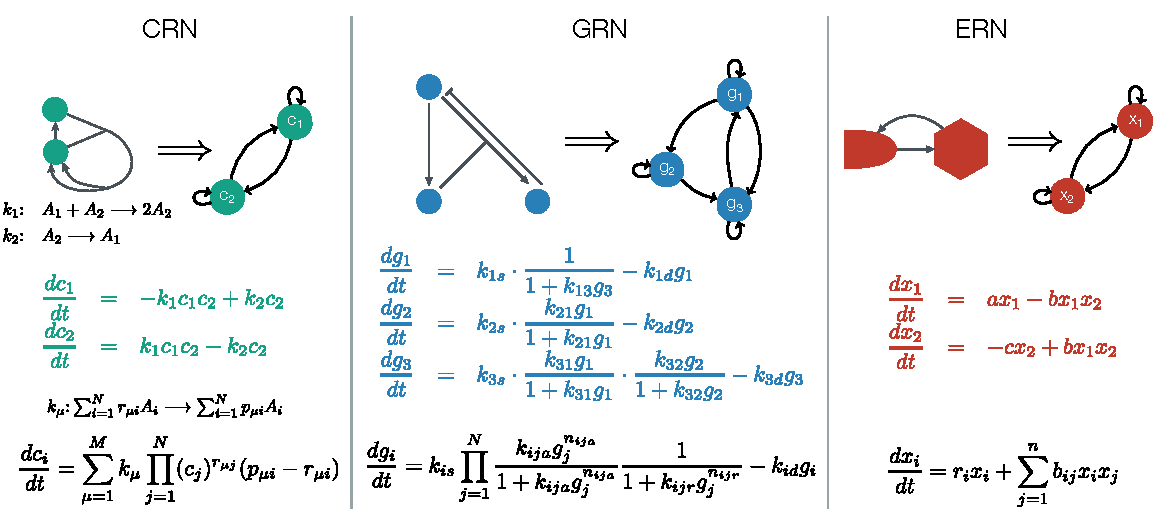
\includegraphics[width=0.8\textwidth]{fig/biomodelexamples.pdf}
\caption{{\bf Dynamical models in systems biology.} The top row represents a chemical reaction network (CRN) \cite{Shinar2010}, a gene regulatory network (GRN) \cite{Karlebach2008}, and an ecological regulatory network (ERN) \cite{Rohr2014} in terms of the graphical methods specific to each field mapped into the interaction graph, which provides a unified representation for networks across these fields. The second row represents a particular example of a system of differential equations that are used to model a biological network within each of the domains of application considered here. The third row shows the general form of a system of differential equations that can be used to model any network architecture within each domain.}
\label{fig:biomodelexamples}
\end{figure*}

\pagebreak

\begin{figure*}[!htbp]
\centering
\noindent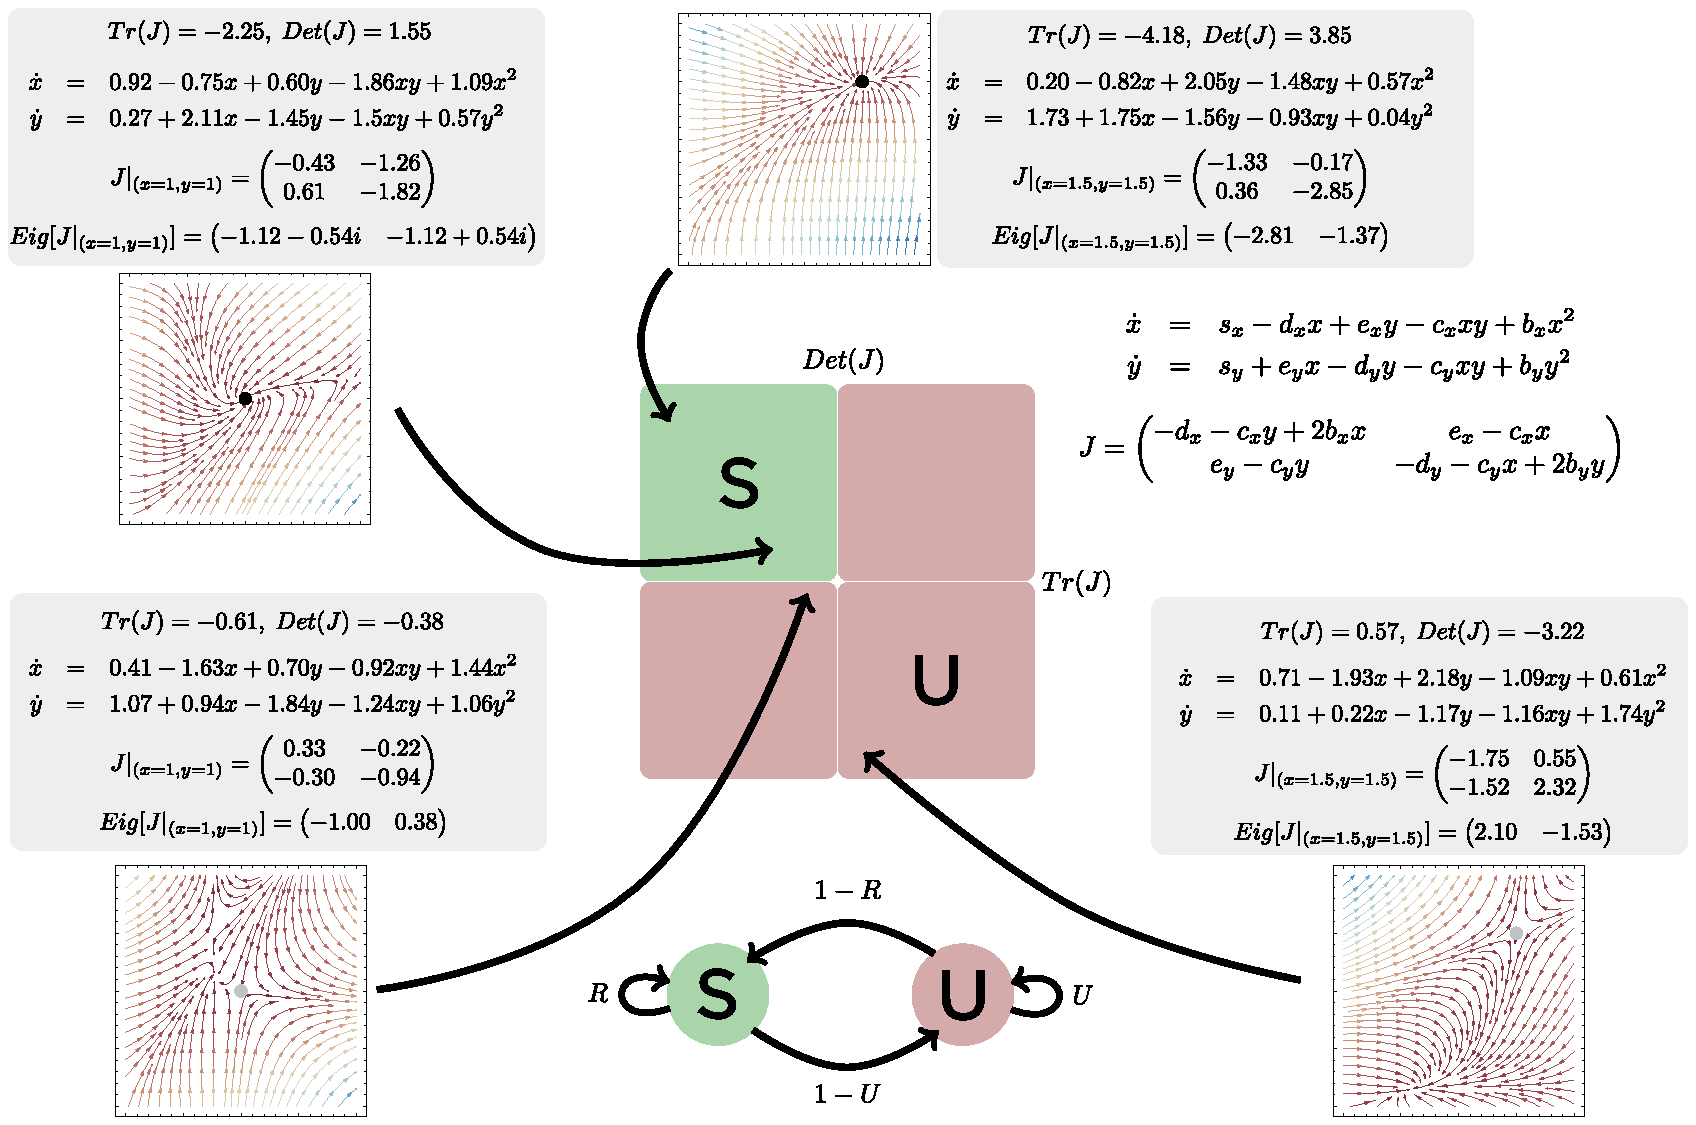
\includegraphics[width=1.0\textwidth]{fig/robustnessconcept.pdf}
\caption{{\bf Stability and robustness of biological networks.} Linearization around a steady-state of a model of a biological network allows for the assessment of the stability of that state. For two-dimensional systems, assessment of stability in terms of the trace and determinant of the Jacobian matrix associated to a particular steady-state geometrically partitions the plane into a stable region (S, blue) and an unstable region (U, red). The stochastic process induced on the stable and unstable regions that results from modifications to a given dynamical model over evolutionary timescales is represented by the state transition diagram (bottom middle). The probability of remaining in the stable region in the context of such modifications, given a previously existing stable network, is then provided by estimating $R$.}
\label{fig:robustnessconcept}
\end{figure*}

\pagebreak

\begin{figure*}[!ht]
\centering
\noindent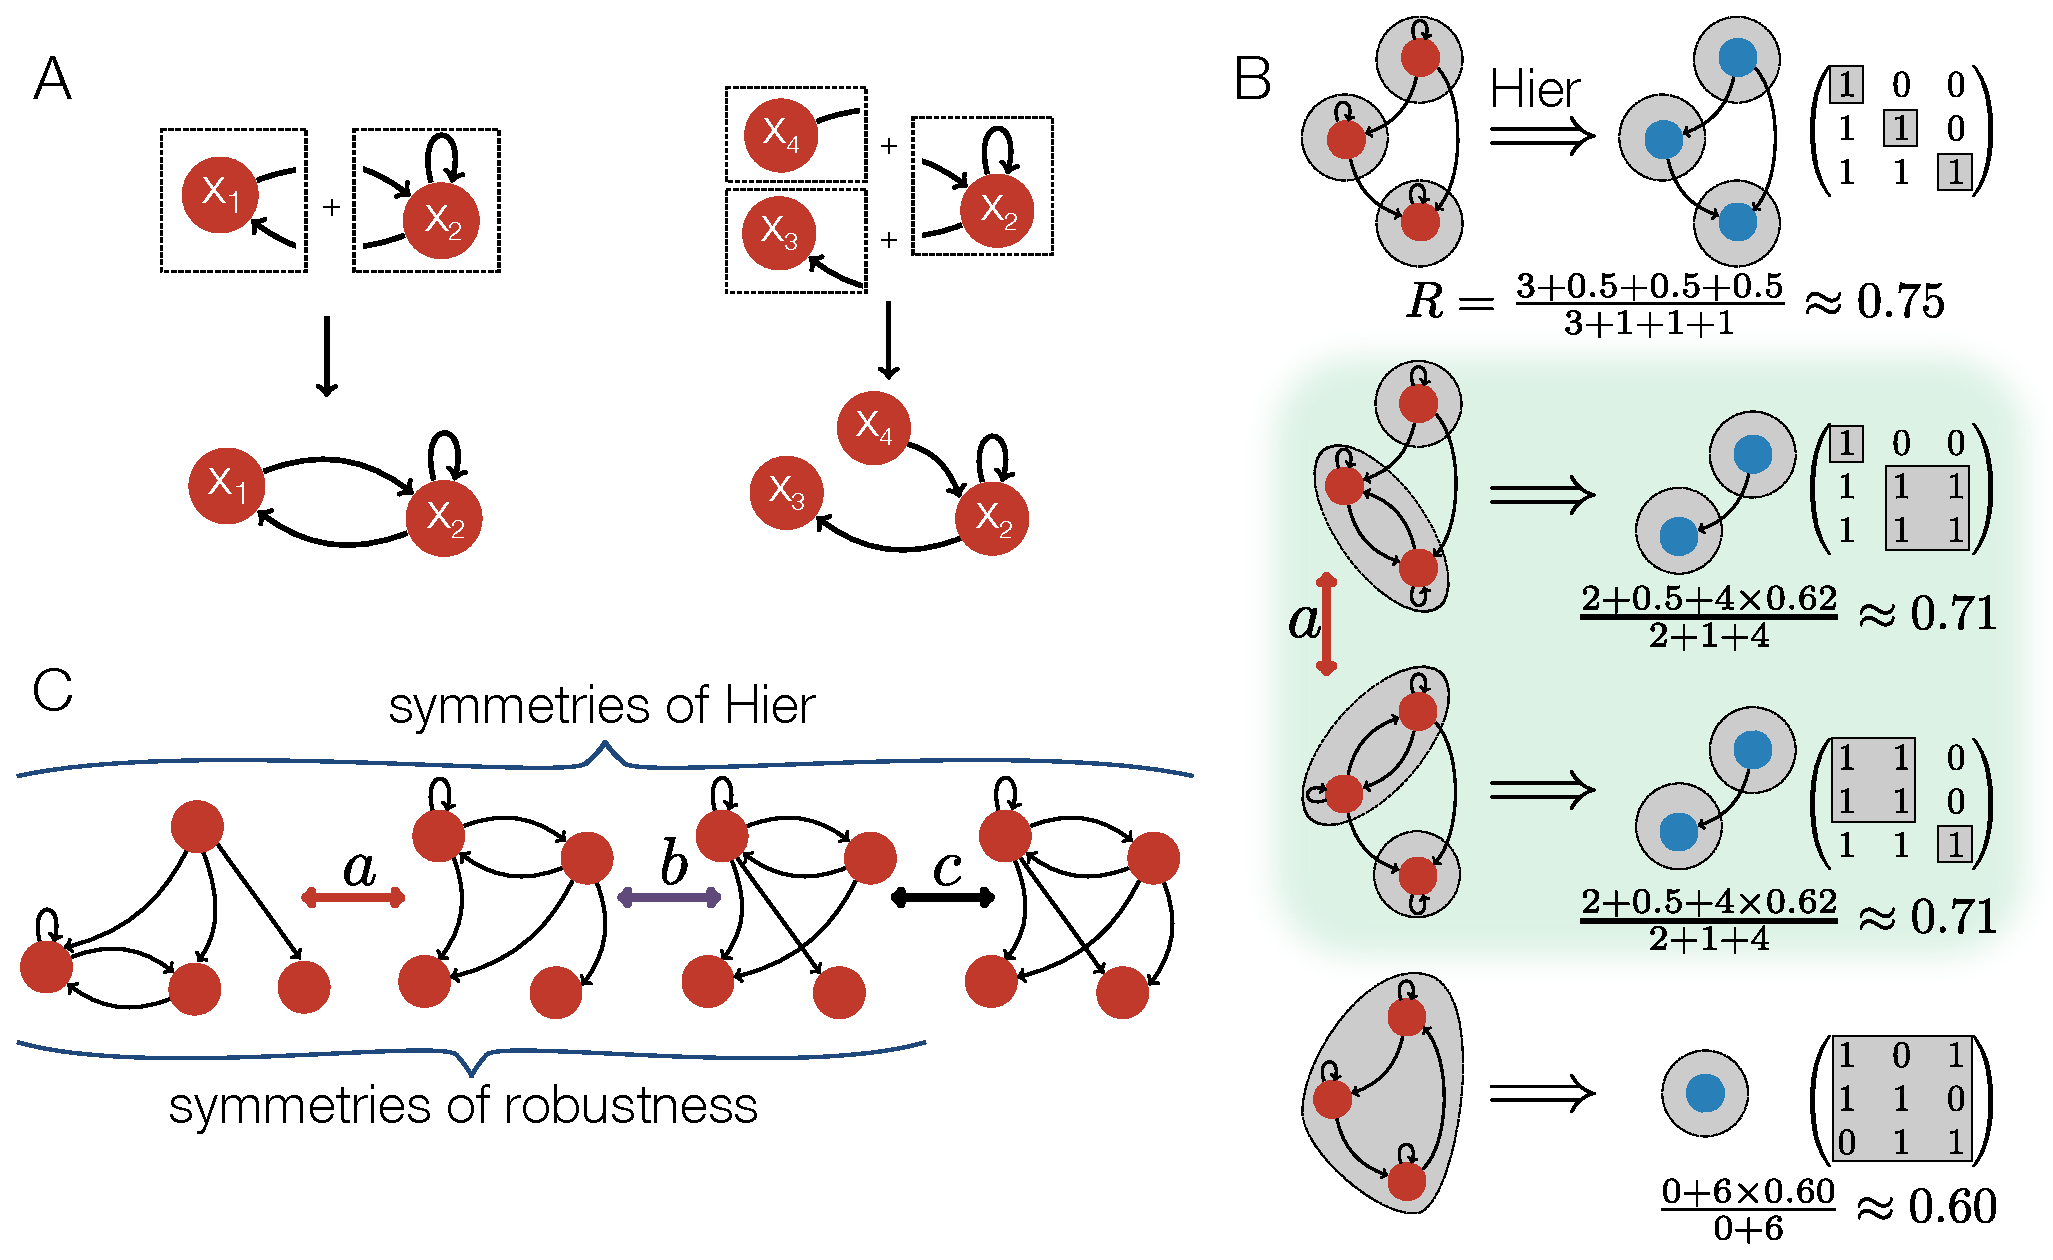
\includegraphics[width=0.8\textwidth]{fig/modsccsym.pdf}
\caption{{\bf Open systems, strongly connected components and symmetries of robustness.} (A) Example of the combination of open system modules to construct closed systems. (B) SCCs highlighted in gray for each of the four graphs representing the interdependencies relevant to four different three variable systems. The most hierarchical network, top panel, is the one that maximizes the number of SCCs and the number of links between them. We therefore define hierarchy as $max(\hbox{ED}) - \hbox{ED}$ where ED is the edit distance representing the number of link addition/deletion operations necessary to transform a given graph into the most hierarchical one. The two panels in the middle represent examples of hierarchical modular systems that posess both modularity (i.e. SCCs with more than one variable) and hierarchy. (C) Symmetries of the $\hier$ transformation between graphs and SCCs. The transformation $a$ represents an interchange of SCCs, $b$ moving a link between nodes in a component and $c$ adding a link. All three transformations represent symmetries of the $\hier$ transformation from graphs to SCCs while only $a$ and $b$ are symmetries of robustness.}
\label{fig:modsccsym}
\end{figure*}

\pagebreak

\begin{figure*}[!ht]
\centering
\noindent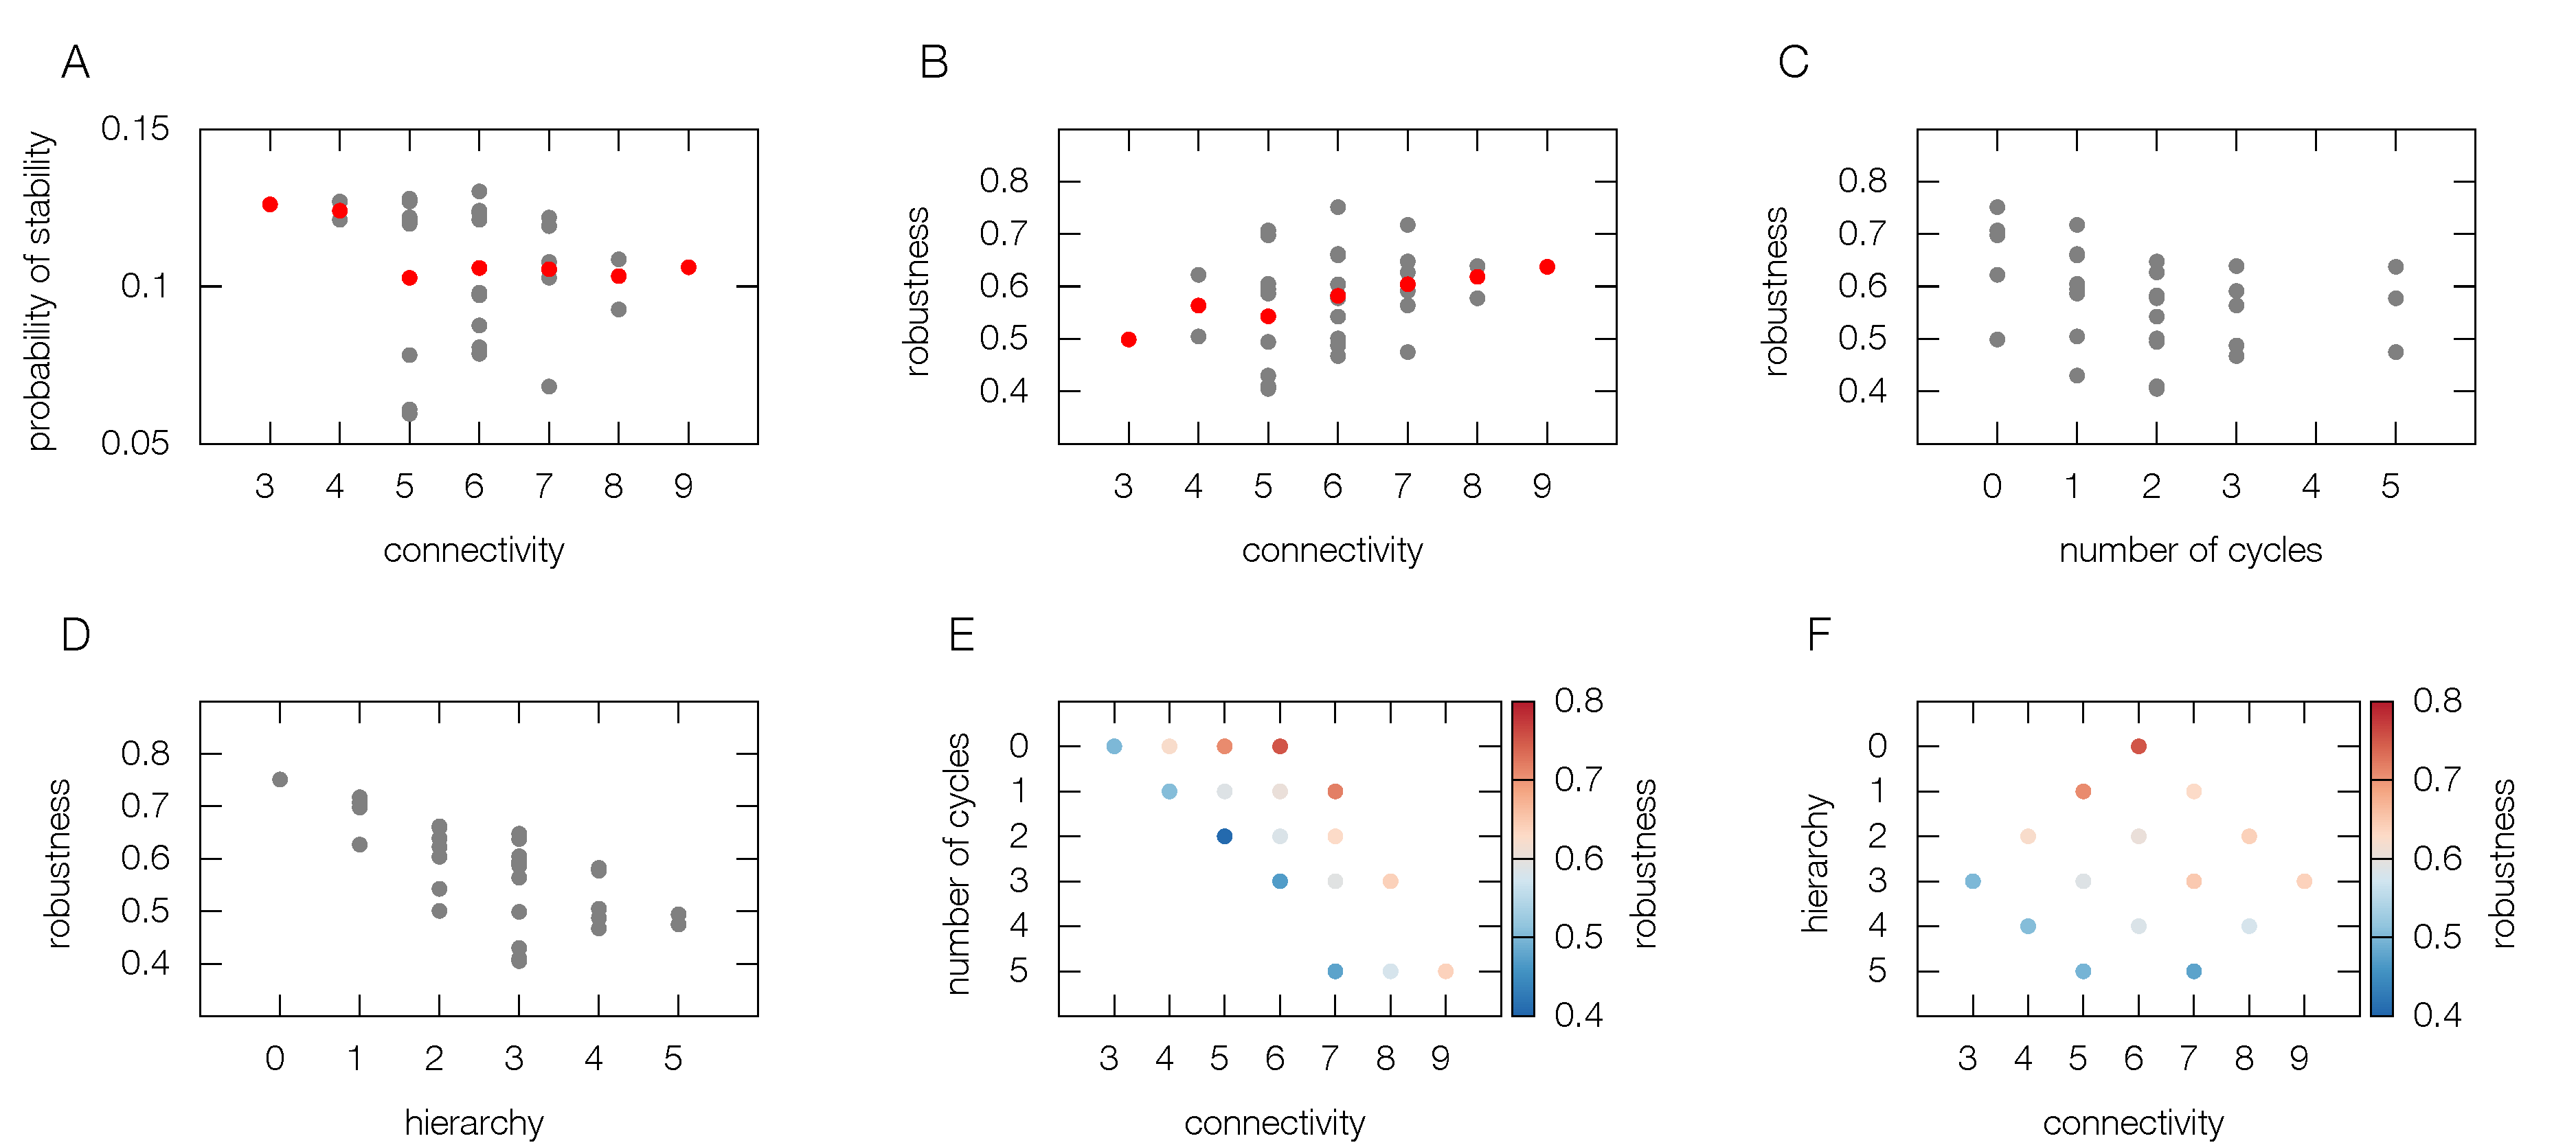
\includegraphics[width=0.8\textwidth]{fig/combinedfigs.pdf}
\caption{{\bf Characterization of stability and robustness according to properties of system structure for three variable systems} (A) Robustness versus connectivity. The red line represents a best fit in the least-squares sense with Pearson product-moment correlation coefficient $r=0.29$. The lowest and highest robustness network architectures are labelled. Other network architectures are shown in \ref{tab:structstabmat3}. (B) Robustness versus hierarchy. Correlation coefficient $r=0.67$. (C) Number of cycles and (D) hierarchy vs connectivity and robustness. The color of each point represents the average robustness of all graphs having the parameters specified on the $x$ and $y$ axes.
}
\label{fig:combined}
\end{figure*}

% \begin{figure}[!ht]
% \centering
% \noindent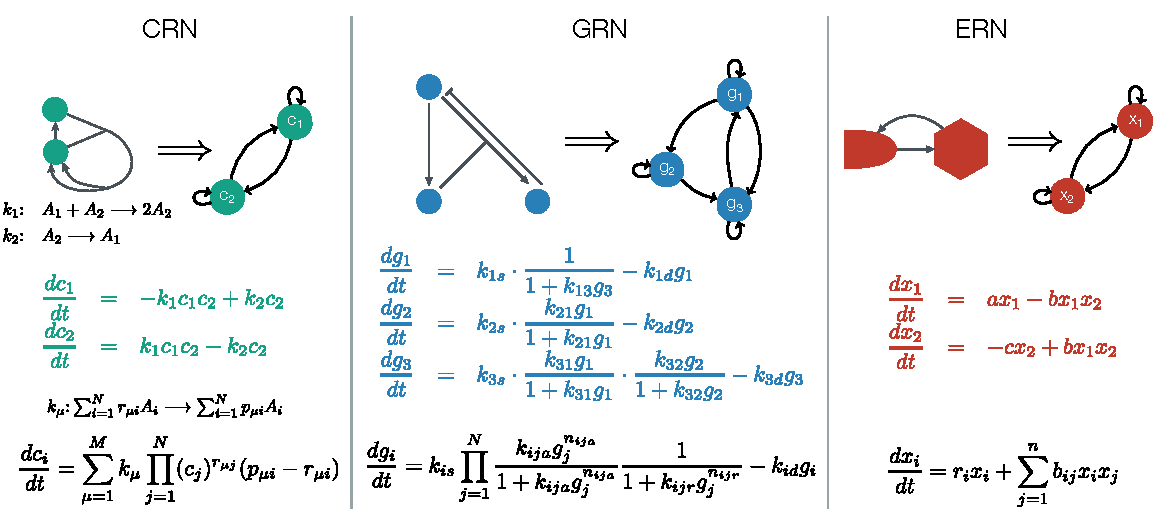
\includegraphics[width=0.9\columnwidth]{fig/biomodelexamples.pdf}
% \caption{{\bf Dynamical models in systems biology.} The top row represents a chemical reaction network (CRN) \cite{Shinar2010}, a gene regulatory network (GRN) \cite{Karlebach2008}, and an ecological regulatory network (ERN) \cite{Rohr2014} in terms of the graphical methods specific to each field mapped into the interaction graph, which provides a unified representation for networks across these fields. The second row represents a particular example of a system of differential equations that are used to model a biological network within each of the domains of application considered here. The third row shows the general form of a system of differential equations that can be used to model any network architecture within each domain.}
% \label{fig:biomodelexamples}
% \end{figure}

% \pagebreak

% \begin{figure}[!ht]
% \centering
% \noindent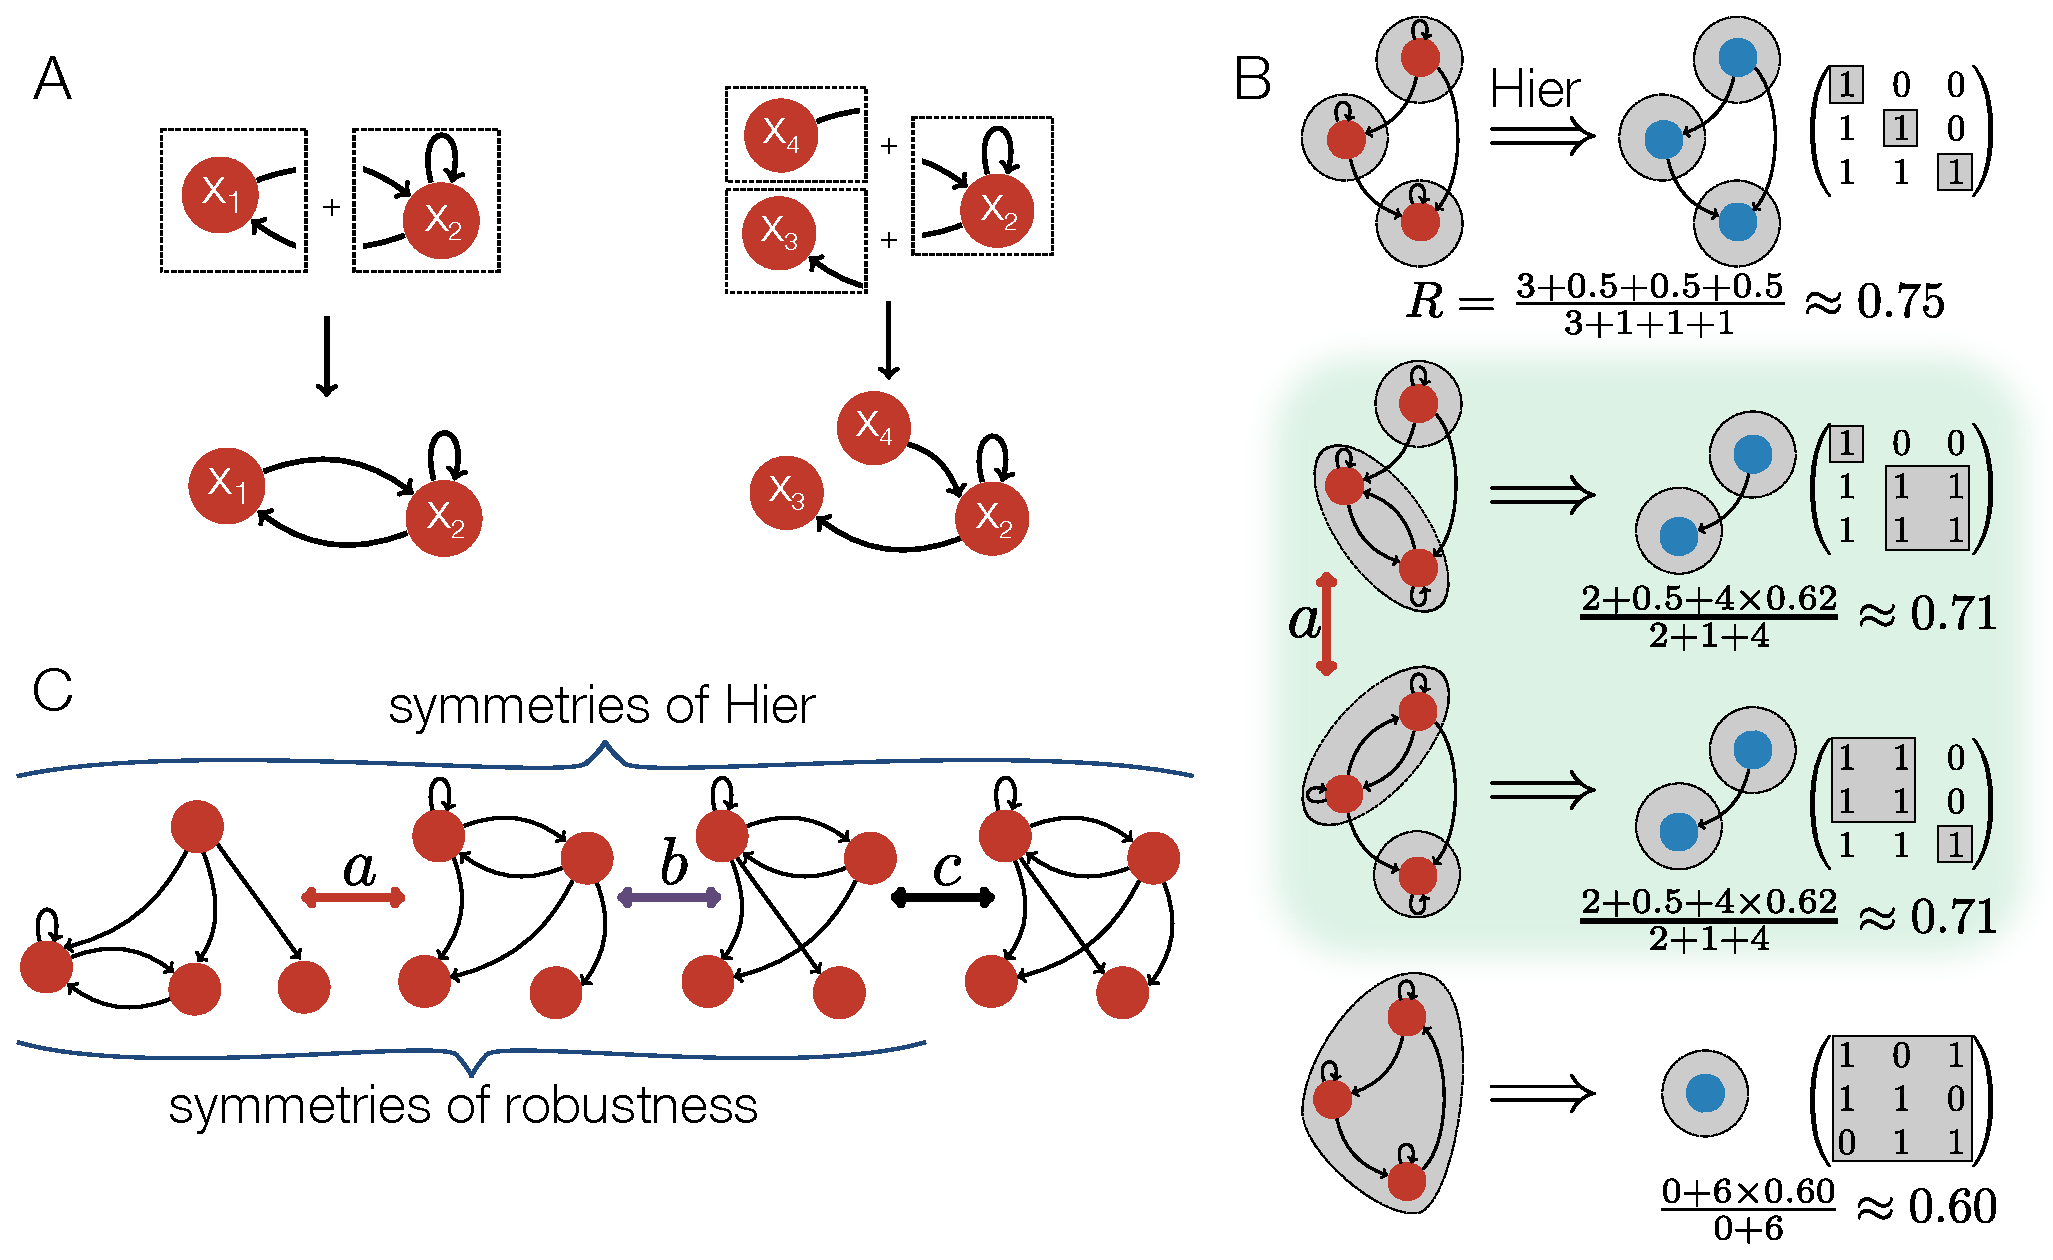
\includegraphics[width=0.9\columnwidth]{fig/modsccsym.pdf}
% \caption{{\bf Open systems, strongly connected components and symmetries of robustness.} (A) Example of the combination of open system modules to construct closed systems. (B) SCCs highlighted in gray for each of the four graphs representing the interdependencies relevant to four different three variable systems. The most hierarchical network, top panel, is the one that maximizes the number of SCCs and the number of links between them. We therefore define hierarchy as $max(\hbox{ED}) - \hbox{ED}$ where ED is the edit distance representing the number of link addition/deletion operations necessary to transform a given graph into the most hierarchical one. The two panels in the middle represent examples of hierarchical modular systems that posess both modularity (i.e. SCCs with more than one variable) and hierarchy. (C) Symmetries of the $\hier$ transformation between graphs and SCCs. The transformation $a$ represents an interchange of SCCs, $b$ moving a link between nodes in a component and $c$ adding a link. All three transformations represent symmetries of the $\hier$ transformation from graphs to SCCs while only $a$ and $b$ are symmetries of robustness.}
% \label{fig:modsccsym}
% \end{figure}

% \pagebreak


% \begin{figure}[!ht]
% \centering
% \noindent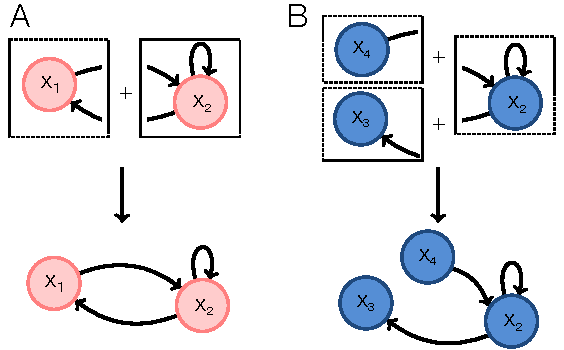
\includegraphics[width=0.4\columnwidth]{fig/examplesystemmodules.pdf}
% \caption{{\bf Example of the combination of open system modules to construct closed systems.} (A) Example of combining two open modules to construct a closed system of two components (B) Analogous example for combining three open modules to construct a closed system with three components}
% \label{fig:examplesystemmodules}
% \end{figure}

% \pagebreak

% \begin{figure}[!ht]
% \centering
% \noindent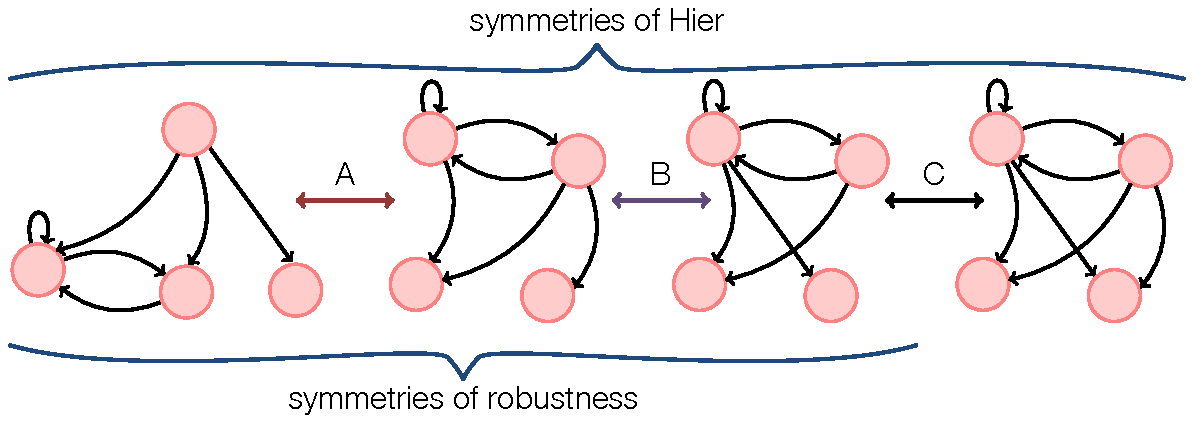
\includegraphics[width=0.7\columnwidth]{fig/hiertransformations.pdf}
% \caption{{\bf Symmetries of the $\hier$ transformation between graphs and SCCs.} The transformation A represents an interchange of SCCs, B moving a link between nodes in a component and C adding a link. All three transformations represent symmetries of the $\hier$ transformation from graphs to SCCs while only A and B are symmetries of robustness.}
% \label{fig:hiertransformations}
% \end{figure}

% \pagebreak

% \begin{figure}[!ht]
% \centering
% \noindent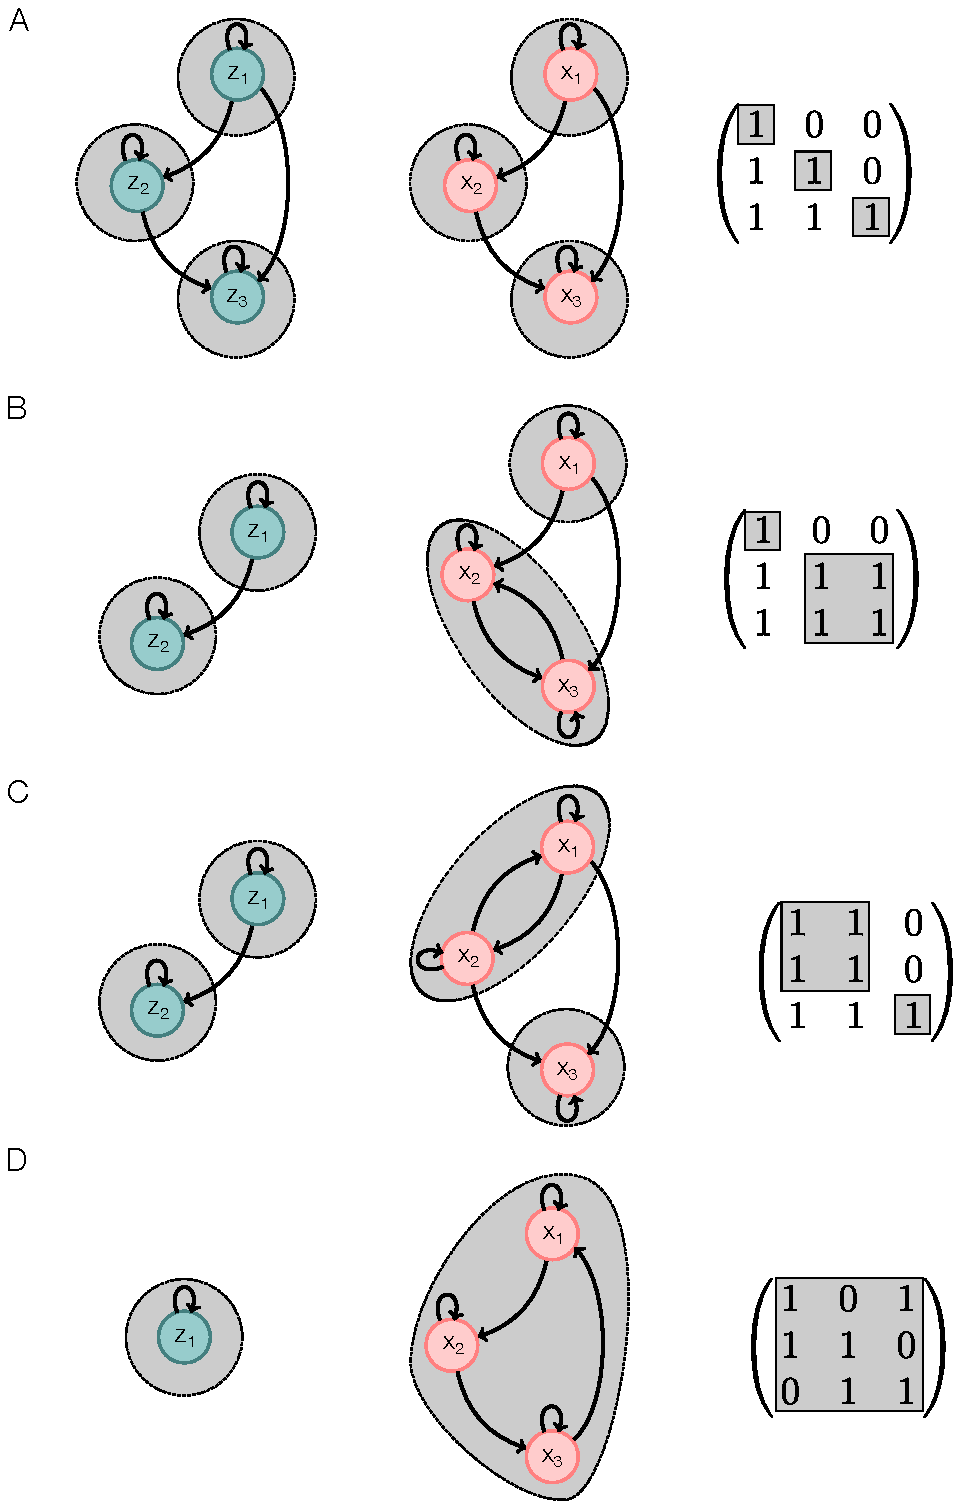
\includegraphics[width=0.4\columnwidth]{fig/scc2.pdf}
% \caption{{\bf Example of strongly connected components.} (A) - (D) show strongly connected components highlighted in gray for each of the four graphs representing the interdependencies relevant to four different three variable systems. Note that the most hierarchical system in (A) has the highest possible number of connected components, three, whereas the system containing a single cycle and therefore posessing no hierarchy contains only one connected component. Systems (B) and (C) represent examples of hierarchical modular systems that posess both modularity and hierarchy.}
% \label{fig:scc}
% \end{figure}

% \pagebreak

% \begin{figure}[!ht]
% \centering
% \noindent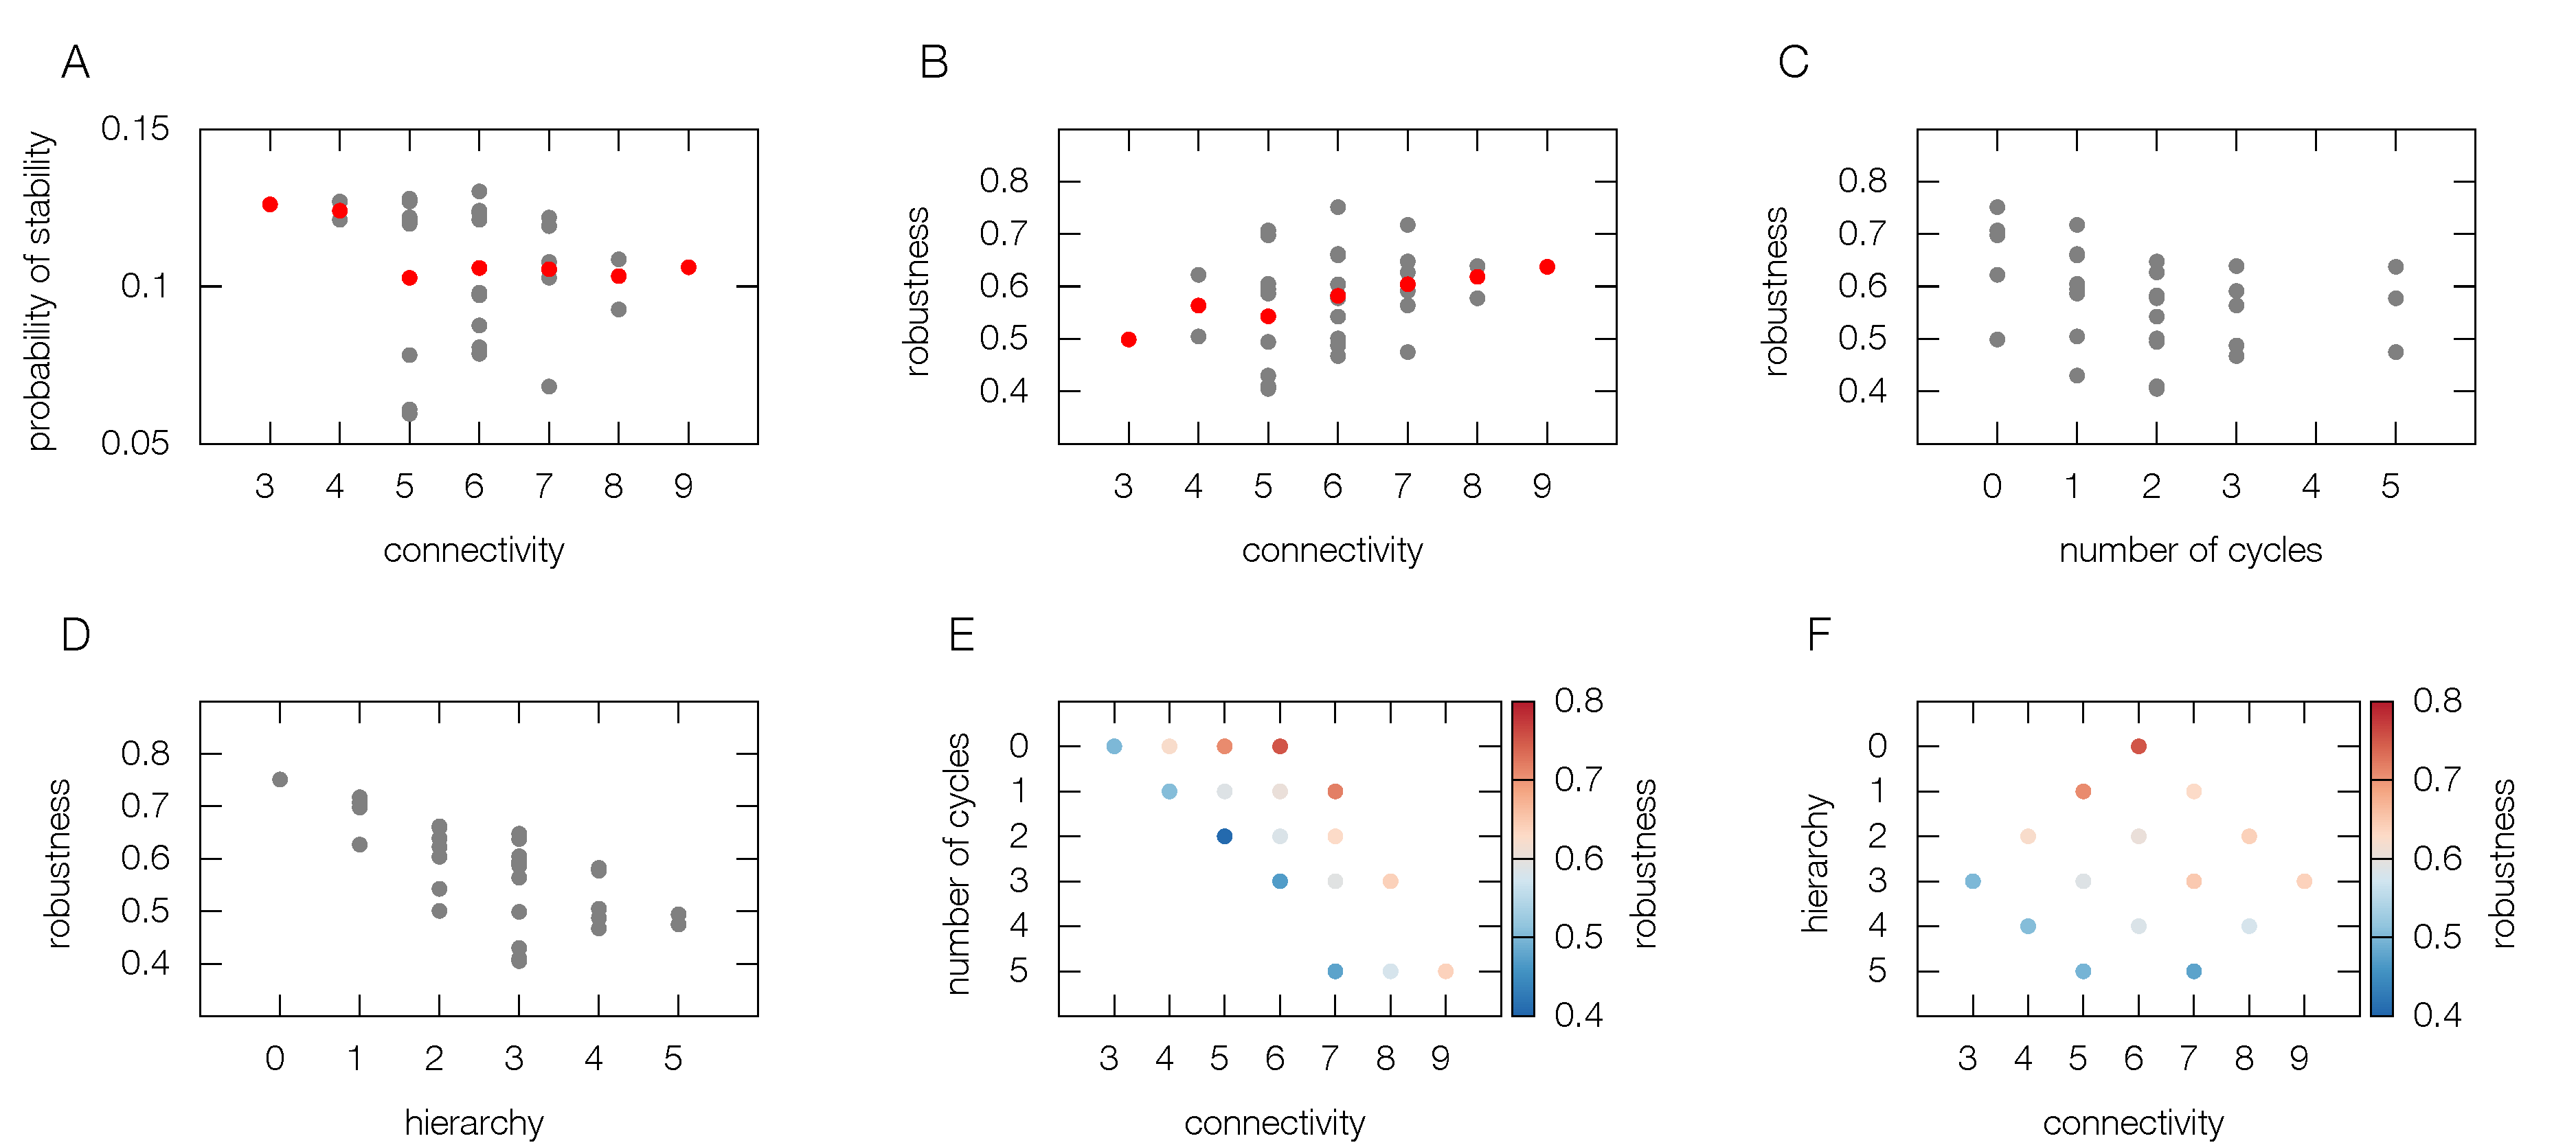
\includegraphics[width=1.0\columnwidth]{fig/combinedfigs.pdf}
% \caption{{\bf Characterization of stability and robustness according to properties of system structure for three variable systems} (A) Robustness versus connectivity. The red line represents a best fit in the least-squares sense with Pearson product-moment correlation coefficient $r=0.29$. The lowest and highest robustness network architectures are labelled. Other network architectures are shown in \ref{tab:structstabmat3}. (B) Robustness versus hierarchy. Correlation coefficient $r=0.67$. (C) Number of cycles and (D) hierarchy vs connectivity and robustness. The color of each point represents the average robustness of all graphs having the parameters specified on the $x$ and $y$ axes.
% }
% \label{fig:combined}
% \end{figure}

% \pagebreak

% \begin{figure}[!ht]
% \centering
% \noindent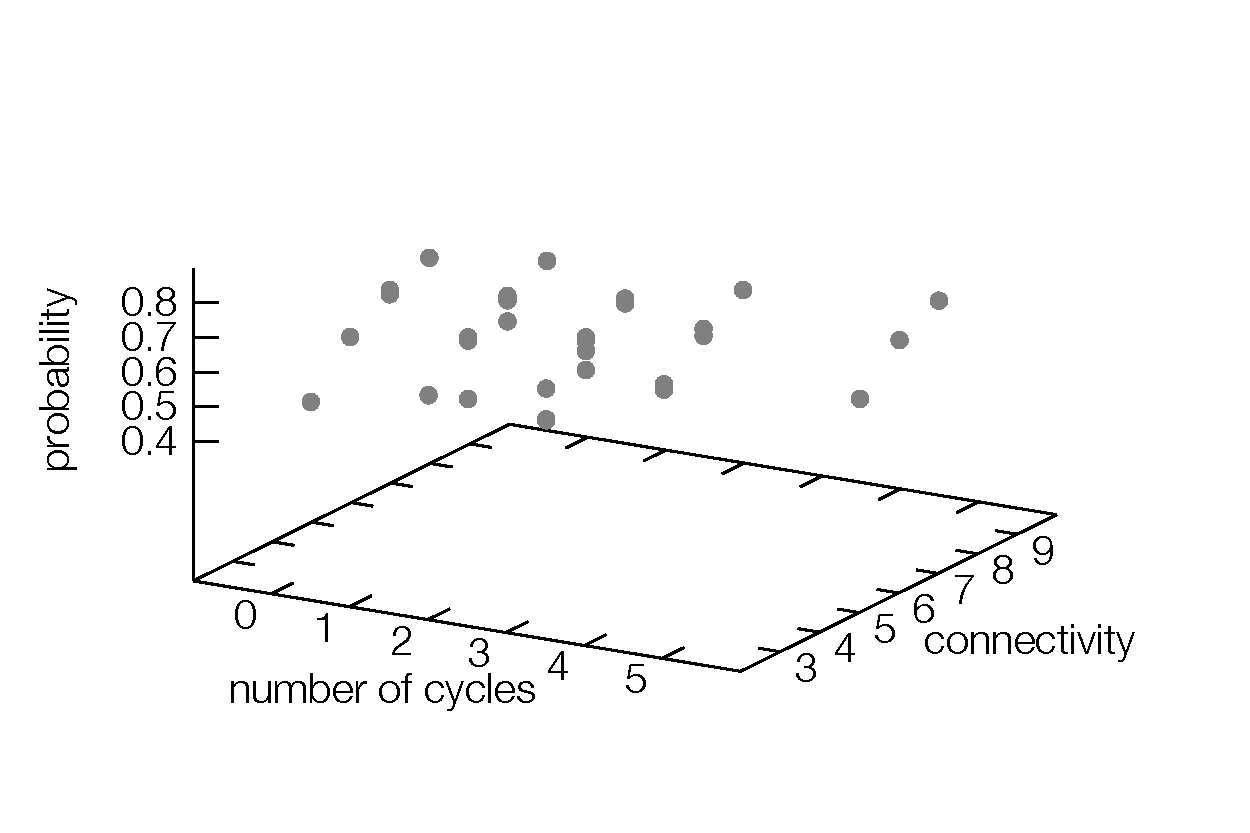
\includegraphics[width=0.8\columnwidth]{fig/connectcycle3D3x3.pdf}
% \caption{{\bf Robustness versus number of cycles and connectivity for three variable systems.} Each point represents the average robustness of all graphs having a given number of cycles and connectivity.}
% \label{fig:connectcycle3D3x3}
% \end{figure}

% \pagebreak

% \begin{figure}[!ht]
% \centering
% \noindent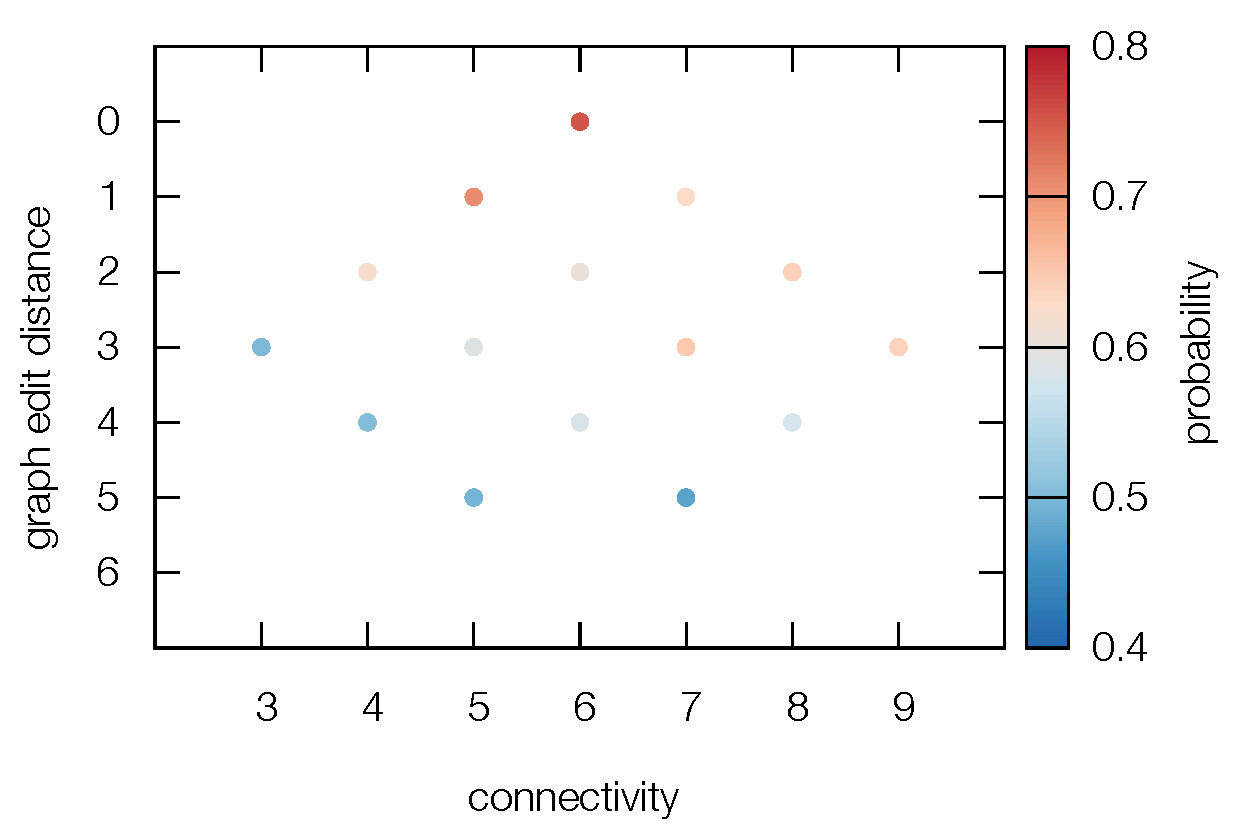
\includegraphics[width=0.8\columnwidth]{fig/connectdist3D3x3.pdf}
% \caption{{\bf Robustness versus hierarchy and connectivity for three variable systems.} Each point represents the average robustness of all graphs having a given hierarchy and connectivity.}
% \label{fig:connectdist3D3x3}
% \end{figure}



\newpage
\FloatBarrier

\section{Tables}
%!TEX root = ../paper.tex
\begin{table}[h]
\begin{center}
\begin{tabular}{ c || c }
\hline
symbol & interpretation\\
\hline
$\connectivity$ & connectivity\\
\end{tabular}
\end{center}
\caption{{\bf Table of notation}.}\label{tab:notation}
\end{table}

%!TEX root = ../paper.tex
\newcommand{\specialcell}[2][c]{%
  \begin{tabular}[#1]{@{}c@{}}#2\end{tabular}}

\begin{table}[h]
\begin{tabular}{ c || c | c | c }
\hline
matrix & connectivity & \specialcell{probability of stability\\to perturbation} & probability of stability\\
\hline
  $\begin{pmatrix}
a & b \\
d & c
\end{pmatrix}$ & 4 & 0.62 & 0.25 \\
  $\begin{pmatrix}
a & b \\
d & 0
\end{pmatrix}$, $\begin{pmatrix}
0 & b \\
d & c
\end{pmatrix}$ & 3 & 0.5 & 0.25 \\
  $\begin{pmatrix}
a & 0 \\
d & c
\end{pmatrix}$, $\begin{pmatrix}
a & b \\
0 & c
\end{pmatrix}$ & 3 & 0.67 & 0.25 \\
$\begin{pmatrix}
a & 0 \\
0 & c
\end{pmatrix}$ & 2 & 0.5 & 0.25 \\
\end{tabular}
\caption{{\bf Probability of stability under resampling and \emph{a priori} stability for two component systems derived analytically}. All matrices not listed have $0$ probability of stability.}\label{tab:structstabmat}
\end{table}

%!TEX root = ../paper.tex
\begin{longtable}{ c | c || c | c | c | c | c }
\hline
matrix & \specialcell{orbit\\size} & connectivity & \specialcell{edit\\distance} & \specialcell{cycle\\number} & \specialcell{probability of stability\\to perturbation} & \specialcell{probability\\of stability}\\
\hline
$\begin{pmatrix}
1 & 0 & 0\\
0 & 1 & 0\\
0 & 0 & 1\\
\end{pmatrix}$ & 1 & 3 & 3 & 0 & 0.499 & 0.126\\
$\begin{pmatrix}
0 & 0 & 1\\
0 & 1 & 0\\
1 & 0 & 1\\
\end{pmatrix}$ & 6 & 4 & 4 & 1 & 0.505 & 0.121\\
$\begin{pmatrix}
1 & 0 & 0\\
0 & 1 & 1\\
0 & 0 & 1\\
\end{pmatrix}$ & 6 & 4 & 2 & 0 & 0.622 & 0.127\\
$\begin{pmatrix}
0 & 0 & 1\\
0 & 1 & 1\\
1 & 0 & 1\\
\end{pmatrix}$ & 12 & 5 & 3 & 1 & 0.595 & 0.121\\
$\begin{pmatrix}
0 & 0 & 1\\
0 & 1 & 1\\
1 & 1 & 0\\
\end{pmatrix}$ & 6 & 5 & 5 & 2 & 0.494 & 0.128\\
$\begin{pmatrix}
0 & 1 & 1\\
0 & 0 & 1\\
1 & 0 & 1\\
\end{pmatrix}$ & 12 & 5 & 3 & 2 & 0.41 & 0.061\\
$\begin{pmatrix}
0 & 1 & 0\\
0 & 1 & 1\\
1 & 0 & 1\\
\end{pmatrix}$ & 6 & 5 & 3 & 1 & 0.43 & 0.078\\
$\begin{pmatrix}
0 & 1 & 1\\
0 & 1 & 0\\
1 & 0 & 1\\
\end{pmatrix}$ & 12 & 5 & 3 & 1 & 0.605 & 0.12\\
$\begin{pmatrix}
0 & 1 & 1\\
0 & 1 & 1\\
1 & 0 & 0\\
\end{pmatrix}$ & 6 & 5 & 3 & 2 & 0.405 & 0.06\\
$\begin{pmatrix}
1 & 0 & 1\\
0 & 1 & 1\\
0 & 0 & 1\\
\end{pmatrix}$ & 6 & 5 & 1 & 0 & 0.698 & 0.122\\
$\begin{pmatrix}
1 & 0 & 0\\
0 & 1 & 1\\
0 & 1 & 1\\
\end{pmatrix}$ & 3 & 5 & 3 & 1 & 0.587 & 0.128\\
$\begin{pmatrix}
1 & 0 & 1\\
0 & 1 & 0\\
0 & 1 & 1\\
\end{pmatrix}$ & 6 & 5 & 1 & 0 & 0.707 & 0.127\\
$\begin{pmatrix}
0 & 0 & 1\\
0 & 1 & 1\\
1 & 1 & 1\\
\end{pmatrix}$ & 6 & 6 & 4 & 2 & 0.578 & 0.121\\
$\begin{pmatrix}
0 & 1 & 1\\
0 & 0 & 1\\
1 & 1 & 1\\
\end{pmatrix}$ & 6 & 6 & 4 & 3 & 0.487 & 0.081\\
$\begin{pmatrix}
0 & 1 & 1\\
0 & 1 & 1\\
1 & 0 & 1\\
\end{pmatrix}$ & 12 & 6 & 2 & 2 & 0.543 & 0.098\\
$\begin{pmatrix}
0 & 1 & 0\\
0 & 1 & 1\\
1 & 1 & 1\\
\end{pmatrix}$ & 6 & 6 & 2 & 2 & 0.501 & 0.088\\
$\begin{pmatrix}
0 & 1 & 1\\
0 & 1 & 0\\
1 & 1 & 1\\
\end{pmatrix}$ & 12 & 6 & 2 & 1 & 0.662 & 0.123\\
$\begin{pmatrix}
0 & 1 & 1\\
0 & 1 & 1\\
1 & 1 & 0\\
\end{pmatrix}$ & 12 & 6 & 4 & 3 & 0.467 & 0.079\\
$\begin{pmatrix}
0 & 1 & 1\\
1 & 1 & 0\\
1 & 0 & 1\\
\end{pmatrix}$ & 3 & 6 & 4 & 2 & 0.583 & 0.13\\
$\begin{pmatrix}
1 & 0 & 1\\
0 & 1 & 1\\
0 & 1 & 1\\
\end{pmatrix}$ & 12 & 6 & 2 & 1 & 0.659 & 0.124\\
$\begin{pmatrix}
1 & 1 & 1\\
0 & 1 & 1\\
0 & 0 & 1\\
\end{pmatrix}$ & 6 & 6 & 0 & 0 & 0.751 & 0.124\\
$\begin{pmatrix}
1 & 1 & 0\\
0 & 1 & 1\\
1 & 0 & 1\\
\end{pmatrix}$ & 2 & 6 & 2 & 1 & 0.604 & 0.097\\
$\begin{pmatrix}
0 & 1 & 1\\
0 & 1 & 1\\
1 & 1 & 1\\
\end{pmatrix}$ & 12 & 7 & 3 & 3 & 0.564 & 0.103\\
$\begin{pmatrix}
0 & 1 & 1\\
1 & 0 & 1\\
1 & 1 & 1\\
\end{pmatrix}$ & 3 & 7 & 5 & 5 & 0.475 & 0.068\\
$\begin{pmatrix}
0 & 1 & 1\\
1 & 1 & 1\\
1 & 0 & 1\\
\end{pmatrix}$ & 6 & 7 & 3 & 3 & 0.591 & 0.108\\
$\begin{pmatrix}
1 & 1 & 1\\
0 & 1 & 1\\
0 & 1 & 1\\
\end{pmatrix}$ & 6 & 7 & 1 & 1 & 0.717 & 0.119\\
$\begin{pmatrix}
1 & 0 & 1\\
0 & 1 & 1\\
1 & 1 & 1\\
\end{pmatrix}$ & 3 & 7 & 3 & 2 & 0.648 & 0.122\\
$\begin{pmatrix}
1 & 1 & 1\\
0 & 1 & 1\\
1 & 0 & 1\\
\end{pmatrix}$ & 6 & 7 & 1 & 2 & 0.627 & 0.105\\
$\begin{pmatrix}
0 & 1 & 1\\
1 & 1 & 1\\
1 & 1 & 1\\
\end{pmatrix}$ & 3 & 8 & 4 & 5 & 0.577 & 0.093\\
$\begin{pmatrix}
1 & 1 & 1\\
0 & 1 & 1\\
1 & 1 & 1\\
\end{pmatrix}$ & 6 & 8 & 2 & 3 & 0.639 & 0.109\\
$\begin{pmatrix}
1 & 1 & 1\\
1 & 1 & 1\\
1 & 1 & 1\\
\end{pmatrix}$ & 1 & 9 & 3 & 5 & 0.638 & 0.106\\
\caption{{\bf Robustness and stability for three component systems estimated via Monte Carlo sampling.} All matrices not listed have $0$ probability of stability.}\label{tab:structstabmat3}
\end{longtable}


% \newpage

% %!TEX root = ../paper.tex
\begin{longtable}{ c || c | c | c | c }
\hline
matrix & connectivity & cycle number & \specialcell{probability of stability\\to perturbation} & probability of stability\\
\hline
\begin{tikzpicture}[scale=0.6,
every state/.style={draw=red!50,very thick,fill=red!20}]
\begin{dot2tex}[styleonly,codeonly,neato,mathmode]
digraph G {
d2ttikzedgelabels = true;
node [style="state"];
edge [lblstyle="auto",topath="bend left",style="line width=1.5pt"];
1 -> 1 [topath="loop above"];
2 -> 2 [topath="loop above"];
3 -> 3 [topath="loop above"];
}
\end{dot2tex}
\end{tikzpicture} & 3 & 0 & 0.499 & 0.126\\
\begin{tikzpicture}[scale=0.6,
every state/.style={draw=red!50,very thick,fill=red!20}]
\begin{dot2tex}[styleonly,codeonly,neato,mathmode]
digraph G {
d2ttikzedgelabels = true;
node [style="state"];
edge [lblstyle="auto",topath="bend left",style="line width=1.5pt"];
3 -> 1;
2 -> 2 [topath="loop above"];
1 -> 3;
3 -> 3 [topath="loop above"];
}
\end{dot2tex}
\end{tikzpicture} & 4 & 1 & 0.505 & 0.121\\
\begin{tikzpicture}[scale=0.6,
every state/.style={draw=red!50,very thick,fill=red!20}]
\begin{dot2tex}[styleonly,codeonly,neato,mathmode]
digraph G {
d2ttikzedgelabels = true;
node [style="state"];
edge [lblstyle="auto",topath="bend left",style="line width=1.5pt"];
1 -> 1 [topath="loop above"];
2 -> 2 [topath="loop above"];
3 -> 2;
3 -> 3 [topath="loop above"];
}
\end{dot2tex}
\end{tikzpicture} & 4 & 0 & 0.622 & 0.127\\
\begin{tikzpicture}[scale=0.6,
every state/.style={draw=red!50,very thick,fill=red!20}]
\begin{dot2tex}[styleonly,codeonly,neato,mathmode]
digraph G {
d2ttikzedgelabels = true;
node [style="state"];
edge [lblstyle="auto",topath="bend left",style="line width=1.5pt"];
3 -> 1;
2 -> 2 [topath="loop above"];
3 -> 2;
1 -> 3;
3 -> 3 [topath="loop above"];
}
\end{dot2tex}
\end{tikzpicture} & 5 & 1 & 0.595 & 0.121\\
\begin{tikzpicture}[scale=0.6,
every state/.style={draw=red!50,very thick,fill=red!20}]
\begin{dot2tex}[styleonly,codeonly,neato,mathmode]
digraph G {
d2ttikzedgelabels = true;
node [style="state"];
edge [lblstyle="auto",topath="bend left",style="line width=1.5pt"];
3 -> 1;
2 -> 2 [topath="loop above"];
3 -> 2;
1 -> 3;
2 -> 3;
}
\end{dot2tex}
\end{tikzpicture} & 5 & 2 & 0.494 & 0.128\\
\begin{tikzpicture}[scale=0.6,
every state/.style={draw=red!50,very thick,fill=red!20}]
\begin{dot2tex}[styleonly,codeonly,neato,mathmode]
digraph G {
d2ttikzedgelabels = true;
node [style="state"];
edge [lblstyle="auto",topath="bend left",style="line width=1.5pt"];
2 -> 1;
3 -> 1;
3 -> 2;
1 -> 3;
3 -> 3 [topath="loop above"];
}
\end{dot2tex}
\end{tikzpicture} & 5 & 2 & 0.41 & 0.061\\
\begin{tikzpicture}[scale=0.6,
every state/.style={draw=red!50,very thick,fill=red!20}]
\begin{dot2tex}[styleonly,codeonly,neato,mathmode]
digraph G {
d2ttikzedgelabels = true;
node [style="state"];
edge [lblstyle="auto",topath="bend left",style="line width=1.5pt"];
2 -> 1;
2 -> 2 [topath="loop above"];
3 -> 2;
1 -> 3;
3 -> 3 [topath="loop above"];
}
\end{dot2tex}
\end{tikzpicture} & 5 & 1 & 0.43 & 0.078\\
\begin{tikzpicture}[scale=0.6,
every state/.style={draw=red!50,very thick,fill=red!20}]
\begin{dot2tex}[styleonly,codeonly,neato,mathmode]
digraph G {
d2ttikzedgelabels = true;
node [style="state"];
edge [lblstyle="auto",topath="bend left",style="line width=1.5pt"];
2 -> 1;
3 -> 1;
2 -> 2 [topath="loop above"];
1 -> 3;
3 -> 3 [topath="loop above"];
}
\end{dot2tex}
\end{tikzpicture} & 5 & 1 & 0.605 & 0.12\\
\begin{tikzpicture}[scale=0.6,
every state/.style={draw=red!50,very thick,fill=red!20}]
\begin{dot2tex}[styleonly,codeonly,neato,mathmode]
digraph G {
d2ttikzedgelabels = true;
node [style="state"];
edge [lblstyle="auto",topath="bend left",style="line width=1.5pt"];
2 -> 1;
3 -> 1;
2 -> 2 [topath="loop above"];
3 -> 2;
1 -> 3;
}
\end{dot2tex}
\end{tikzpicture} & 5 & 2 & 0.405 & 0.06\\
\begin{tikzpicture}[scale=0.6,
every state/.style={draw=red!50,very thick,fill=red!20}]
\begin{dot2tex}[styleonly,codeonly,neato,mathmode]
digraph G {
d2ttikzedgelabels = true;
node [style="state"];
edge [lblstyle="auto",topath="bend left",style="line width=1.5pt"];
1 -> 1 [topath="loop above"];
3 -> 1;
2 -> 2 [topath="loop above"];
3 -> 2;
3 -> 3 [topath="loop above"];
}
\end{dot2tex}
\end{tikzpicture} & 5 & 0 & 0.698 & 0.122\\
\begin{tikzpicture}[scale=0.6,
every state/.style={draw=red!50,very thick,fill=red!20}]
\begin{dot2tex}[styleonly,codeonly,neato,mathmode]
digraph G {
d2ttikzedgelabels = true;
node [style="state"];
edge [lblstyle="auto",topath="bend left",style="line width=1.5pt"];
1 -> 1 [topath="loop above"];
2 -> 2 [topath="loop above"];
3 -> 2;
2 -> 3;
3 -> 3 [topath="loop above"];
}
\end{dot2tex}
\end{tikzpicture} & 5 & 1 & 0.587 & 0.128\\
\begin{tikzpicture}[scale=0.6,
every state/.style={draw=red!50,very thick,fill=red!20}]
\begin{dot2tex}[styleonly,codeonly,neato,mathmode]
digraph G {
d2ttikzedgelabels = true;
node [style="state"];
edge [lblstyle="auto",topath="bend left",style="line width=1.5pt"];
1 -> 1 [topath="loop above"];
3 -> 1;
2 -> 2 [topath="loop above"];
2 -> 3;
3 -> 3 [topath="loop above"];
}
\end{dot2tex}
\end{tikzpicture} & 5 & 0 & 0.707 & 0.127\\
\begin{tikzpicture}[scale=0.6,
every state/.style={draw=red!50,very thick,fill=red!20}]
\begin{dot2tex}[styleonly,codeonly,neato,mathmode]
digraph G {
d2ttikzedgelabels = true;
node [style="state"];
edge [lblstyle="auto",topath="bend left",style="line width=1.5pt"];
3 -> 1;
2 -> 2 [topath="loop above"];
3 -> 2;
1 -> 3;
2 -> 3;
3 -> 3 [topath="loop above"];
}
\end{dot2tex}
\end{tikzpicture} & 6 & 2 & 0.578 & 0.121\\
\begin{tikzpicture}[scale=0.6,
every state/.style={draw=red!50,very thick,fill=red!20}]
\begin{dot2tex}[styleonly,codeonly,neato,mathmode]
digraph G {
d2ttikzedgelabels = true;
node [style="state"];
edge [lblstyle="auto",topath="bend left",style="line width=1.5pt"];
2 -> 1;
3 -> 1;
3 -> 2;
1 -> 3;
2 -> 3;
3 -> 3 [topath="loop above"];
}
\end{dot2tex}
\end{tikzpicture} & 6 & 3 & 0.487 & 0.081\\
\begin{tikzpicture}[scale=0.6,
every state/.style={draw=red!50,very thick,fill=red!20}]
\begin{dot2tex}[styleonly,codeonly,neato,mathmode]
digraph G {
d2ttikzedgelabels = true;
node [style="state"];
edge [lblstyle="auto",topath="bend left",style="line width=1.5pt"];
2 -> 1;
3 -> 1;
2 -> 2 [topath="loop above"];
3 -> 2;
1 -> 3;
3 -> 3 [topath="loop above"];
}
\end{dot2tex}
\end{tikzpicture} & 6 & 2 & 0.543 & 0.098\\
\begin{tikzpicture}[scale=0.6,
every state/.style={draw=red!50,very thick,fill=red!20}]
\begin{dot2tex}[styleonly,codeonly,neato,mathmode]
digraph G {
d2ttikzedgelabels = true;
node [style="state"];
edge [lblstyle="auto",topath="bend left",style="line width=1.5pt"];
2 -> 1;
2 -> 2 [topath="loop above"];
3 -> 2;
1 -> 3;
2 -> 3;
3 -> 3 [topath="loop above"];
}
\end{dot2tex}
\end{tikzpicture} & 6 & 2 & 0.501 & 0.088\\
\begin{tikzpicture}[scale=0.6,
every state/.style={draw=red!50,very thick,fill=red!20}]
\begin{dot2tex}[styleonly,codeonly,neato,mathmode]
digraph G {
d2ttikzedgelabels = true;
node [style="state"];
edge [lblstyle="auto",topath="bend left",style="line width=1.5pt"];
2 -> 1;
3 -> 1;
2 -> 2 [topath="loop above"];
1 -> 3;
2 -> 3;
3 -> 3 [topath="loop above"];
}
\end{dot2tex}
\end{tikzpicture} & 6 & 1 & 0.662 & 0.123\\
\begin{tikzpicture}[scale=0.6,
every state/.style={draw=red!50,very thick,fill=red!20}]
\begin{dot2tex}[styleonly,codeonly,neato,mathmode]
digraph G {
d2ttikzedgelabels = true;
node [style="state"];
edge [lblstyle="auto",topath="bend left",style="line width=1.5pt"];
2 -> 1;
3 -> 1;
2 -> 2 [topath="loop above"];
3 -> 2;
1 -> 3;
2 -> 3;
}
\end{dot2tex}
\end{tikzpicture} & 6 & 3 & 0.467 & 0.079\\
\begin{tikzpicture}[scale=0.6,
every state/.style={draw=red!50,very thick,fill=red!20}]
\begin{dot2tex}[styleonly,codeonly,neato,mathmode]
digraph G {
d2ttikzedgelabels = true;
node [style="state"];
edge [lblstyle="auto",topath="bend left",style="line width=1.5pt"];
2 -> 1;
3 -> 1;
1 -> 2;
2 -> 2 [topath="loop above"];
1 -> 3;
3 -> 3 [topath="loop above"];
}
\end{dot2tex}
\end{tikzpicture} & 6 & 2 & 0.583 & 0.13\\
\begin{tikzpicture}[scale=0.6,
every state/.style={draw=red!50,very thick,fill=red!20}]
\begin{dot2tex}[styleonly,codeonly,neato,mathmode]
digraph G {
d2ttikzedgelabels = true;
node [style="state"];
edge [lblstyle="auto",topath="bend left",style="line width=1.5pt"];
1 -> 1 [topath="loop above"];
3 -> 1;
2 -> 2 [topath="loop above"];
3 -> 2;
2 -> 3;
3 -> 3 [topath="loop above"];
}
\end{dot2tex}
\end{tikzpicture} & 6 & 1 & 0.659 & 0.124\\
\begin{tikzpicture}[scale=0.6,
every state/.style={draw=red!50,very thick,fill=red!20}]
\begin{dot2tex}[styleonly,codeonly,neato,mathmode]
digraph G {
d2ttikzedgelabels = true;
node [style="state"];
edge [lblstyle="auto",topath="bend left",style="line width=1.5pt"];
1 -> 1 [topath="loop above"];
2 -> 1;
3 -> 1;
2 -> 2 [topath="loop above"];
3 -> 2;
3 -> 3 [topath="loop above"];
}
\end{dot2tex}
\end{tikzpicture} & 6 & 0 & 0.751 & 0.124\\
\begin{tikzpicture}[scale=0.6,
every state/.style={draw=red!50,very thick,fill=red!20}]
\begin{dot2tex}[styleonly,codeonly,neato,mathmode]
digraph G {
d2ttikzedgelabels = true;
node [style="state"];
edge [lblstyle="auto",topath="bend left",style="line width=1.5pt"];
1 -> 1 [topath="loop above"];
2 -> 1;
2 -> 2 [topath="loop above"];
3 -> 2;
1 -> 3;
3 -> 3 [topath="loop above"];
}
\end{dot2tex}
\end{tikzpicture} & 6 & 1 & 0.604 & 0.097\\
\begin{tikzpicture}[scale=0.6,
every state/.style={draw=red!50,very thick,fill=red!20}]
\begin{dot2tex}[styleonly,codeonly,neato,mathmode]
digraph G {
d2ttikzedgelabels = true;
node [style="state"];
edge [lblstyle="auto",topath="bend left",style="line width=1.5pt"];
2 -> 1;
3 -> 1;
2 -> 2 [topath="loop above"];
3 -> 2;
1 -> 3;
2 -> 3;
3 -> 3 [topath="loop above"];
}
\end{dot2tex}
\end{tikzpicture} & 7 & 3 & 0.564 & 0.103\\
\begin{tikzpicture}[scale=0.6,
every state/.style={draw=red!50,very thick,fill=red!20}]
\begin{dot2tex}[styleonly,codeonly,neato,mathmode]
digraph G {
d2ttikzedgelabels = true;
node [style="state"];
edge [lblstyle="auto",topath="bend left",style="line width=1.5pt"];
2 -> 1;
3 -> 1;
1 -> 2;
3 -> 2;
1 -> 3;
2 -> 3;
3 -> 3 [topath="loop above"];
}
\end{dot2tex}
\end{tikzpicture} & 7 & 5 & 0.475 & 0.068\\
\begin{tikzpicture}[scale=0.6,
every state/.style={draw=red!50,very thick,fill=red!20}]
\begin{dot2tex}[styleonly,codeonly,neato,mathmode]
digraph G {
d2ttikzedgelabels = true;
node [style="state"];
edge [lblstyle="auto",topath="bend left",style="line width=1.5pt"];
2 -> 1;
3 -> 1;
1 -> 2;
2 -> 2 [topath="loop above"];
3 -> 2;
1 -> 3;
3 -> 3 [topath="loop above"];
}
\end{dot2tex}
\end{tikzpicture} & 7 & 3 & 0.591 & 0.108\\
\begin{tikzpicture}[scale=0.6,
every state/.style={draw=red!50,very thick,fill=red!20}]
\begin{dot2tex}[styleonly,codeonly,neato,mathmode]
digraph G {
d2ttikzedgelabels = true;
node [style="state"];
edge [lblstyle="auto",topath="bend left",style="line width=1.5pt"];
1 -> 1 [topath="loop above"];
2 -> 1;
3 -> 1;
2 -> 2 [topath="loop above"];
3 -> 2;
2 -> 3;
3 -> 3 [topath="loop above"];
}
\end{dot2tex}
\end{tikzpicture} & 7 & 1 & 0.717 & 0.119\\
\begin{tikzpicture}[scale=0.6,
every state/.style={draw=red!50,very thick,fill=red!20}]
\begin{dot2tex}[styleonly,codeonly,neato,mathmode]
digraph G {
d2ttikzedgelabels = true;
node [style="state"];
edge [lblstyle="auto",topath="bend left",style="line width=1.5pt"];
1 -> 1 [topath="loop above"];
3 -> 1;
2 -> 2 [topath="loop above"];
3 -> 2;
1 -> 3;
2 -> 3;
3 -> 3 [topath="loop above"];
}
\end{dot2tex}
\end{tikzpicture} & 7 & 2 & 0.648 & 0.122\\
\begin{tikzpicture}[scale=0.6,
every state/.style={draw=red!50,very thick,fill=red!20}]
\begin{dot2tex}[styleonly,codeonly,neato,mathmode]
digraph G {
d2ttikzedgelabels = true;
node [style="state"];
edge [lblstyle="auto",topath="bend left",style="line width=1.5pt"];
1 -> 1 [topath="loop above"];
2 -> 1;
3 -> 1;
2 -> 2 [topath="loop above"];
3 -> 2;
1 -> 3;
3 -> 3 [topath="loop above"];
}
\end{dot2tex}
\end{tikzpicture} & 7 & 2 & 0.627 & 0.105\\
\begin{tikzpicture}[scale=0.6,
every state/.style={draw=red!50,very thick,fill=red!20}]
\begin{dot2tex}[styleonly,codeonly,neato,mathmode]
digraph G {
d2ttikzedgelabels = true;
node [style="state"];
edge [lblstyle="auto",topath="bend left",style="line width=1.5pt"];
2 -> 1;
3 -> 1;
1 -> 2;
2 -> 2 [topath="loop above"];
3 -> 2;
1 -> 3;
2 -> 3;
3 -> 3 [topath="loop above"];
}
\end{dot2tex}
\end{tikzpicture} & 8 & 5 & 0.577 & 0.093\\
\begin{tikzpicture}[scale=0.6,
every state/.style={draw=red!50,very thick,fill=red!20}]
\begin{dot2tex}[styleonly,codeonly,neato,mathmode]
digraph G {
d2ttikzedgelabels = true;
node [style="state"];
edge [lblstyle="auto",topath="bend left",style="line width=1.5pt"];
1 -> 1 [topath="loop above"];
2 -> 1;
3 -> 1;
2 -> 2 [topath="loop above"];
3 -> 2;
1 -> 3;
2 -> 3;
3 -> 3 [topath="loop above"];
}
\end{dot2tex}
\end{tikzpicture} & 8 & 3 & 0.639 & 0.109\\
\begin{tikzpicture}[scale=0.6,
every state/.style={draw=red!50,very thick,fill=red!20}]
\begin{dot2tex}[styleonly,codeonly,neato,mathmode]
digraph G {
d2ttikzedgelabels = true;
node [style="state"];
edge [lblstyle="auto",topath="bend left",style="line width=1.5pt"];
1 -> 1 [topath="loop above"];
2 -> 1;
3 -> 1;
1 -> 2;
2 -> 2 [topath="loop above"];
3 -> 2;
1 -> 3;
2 -> 3;
3 -> 3 [topath="loop above"];
}
\end{dot2tex}
\end{tikzpicture} & 9 & 5 & 0.638 & 0.106\\
\caption{{\bf Probability of stability under resampling and \emph{a priori} stability for three variable systems estimated via Monte Carlo sampling.} All matrices not listed have $0$ probability of stability.}\label{tab:structstabmat3graph}
\end{longtable}


\section{Stability criteria}
% \todo{Since there is no point in publishing proofs of results contemporary with Darwin's Origin of Species, this section will be replaced with a reference to Gantmacher.}
Suppose that $M$ is an $n \times n$ matrix with real coefficients.
As previously described, we call
the matrix $M$ stable if all its eigenvalues have negative real part.
Define the characteristic polynomial as $\chi(M)(z) = \det(zI - M)$.
Denote the coefficients of $\chi(M)$ as $s_j$ and its roots as $r_j$,
writing $p(x) = x^n + \sum_{k=1}^n s_k x^{n-k} = \prod_{k=1}^n (x-r_k)$.
Then, since the roots of $\chi$ are the eigenvalues of $M$, asking that
$M$ be stable is equivalent to asking that the roots of $\chi$ all have
negative real part.  Hence, let us call a polynomial stable if all its
roots have negative real part.  We will formulate conditions for this to
happen in terms of the coefficients of $\chi$.

\begin{lemma}
If $M$ is stable, then $s_i > 0$ for all $i$ between $1$ and $n$.
\end{lemma}

\begin{proof}
Assume that $M$ is stable and that it has $2m$ complex roots which come in
complex conjugate pairs and $n-m$ real roots.  Let $r_1 \ldots, r_{2m}$ be
the complex roots with $r_{2k+1}$ being the complex conjugate of $r_{2k}$
and let $r_{2m+1}, \ldots,  r_{n}$ be the real roots. Then we can write the
factorization as follows:
\[
\chi(M)(z) = \prod_{k=1}^{m} (z^2 - (r_{2k} + r_{2k+1}) z + r_{2k} r_{2k+1})
             \prod_{k=2m+1}^{n} (z - r_k)
\]
Since $r_{2k}$ and $r_{2k+1}$ are complex conjugates, $r_{2k} + r_{2k+1} =
\Re r_{2k} = \Re r_{2k+1}$ and $r_{k} r_{2k+1} > 0$.   Since all the
roots have negative real part, all the coefficients of the terms in
the products above are positive so, when we multiply out the product,
we will have all positive terms.  Hence, we conclude that a necessary
condition for $M$ to be stable is that $s_k > 0$ for all $k$.
\end{proof}

To state the next criterion, we will require the quantity $\Delta$, which
is defined as $\prod_{j=1}^{n-1} \prod_{k=j+1}^n (r_1 + r_j)$.  Since
this expression is invariant under permuting the roots, it may be expressed
as a function of the coefficients $s_i$; for small values of $n$, the
resulting expression looks as follows:
\begin{align*}
n=2 \qquad &\Delta = s_1 \\
n=3 \qquad &\Delta = s_3 - s_1 s_2 \\
n=4 \qquad &\Delta = s_1 s_2 s_3 - s_3^2 - s_1^2 s_4 \\
n=5 \qquad &\Delta = s_1 s_2 s_3 s_4 - s_3^2 s_4 - s_1^2 s_4^2 -
                     s_1 s_2^2 s_5 + s_2 s_3 s_5 + 2 s_1 s_4 s_5 - s_5^2
\end{align*}

\begin{lemma}
If a point lies on the boundary of the set of stable polynomials, then
either $s_n = 0$ and $\Delta = 0$.
\end{lemma}

\begin{proof}
Let $S_n$ denote the symmetric group on $n$ objects and let $f \colon
\mathbb{C}^n/S_n \to \mathbb{C}^n$ be the map that sends a set of roots
to the n-tuplet of coefficients of a polynomial.  This map is explicitly
given by the elemetary symmetric polynomials.  By the fundamental theorem
of algebra, it is invertible and, by ???, its inverse is continuous.

Suppose that $p$ is a stable polynomial.  By definition, this means that
$\Re r > 0$ for every root $r$ of $p$.  Since the set $\{r \mid \Re r > 0\}$
is an open subset of $\mathbb{C}^n/S_n$, the continuity of $f^{-1}$ implies
that the set of stable polynomials is open.  Likewise, the set of unstable
polynomials none of whose roots have real part equal to zero is open.

Hence, if a point lies on the boundary of the stable region, it must
correspond to a polynomial with at least one root whose real part is zero.
There are two ways this could happen.  If the root is real, then having
zero real part is the same as the root being zero, hence $s_n = 0$.  If
the root is complex, then having zero real part means that the root and
its complex conjugate are purely imaginary and sum to zero, hence $\Delta = 0$.
\end{proof}

\begin{lemma}
If $n < 6$, then a polynomial $p$ is stable if and only
if $\Delta > 0$ and $s_1 > 0$ for all $i$.
\end{lemma}

\begin{proof}
Suppose that, to the contrary, there exists a polynomial which satisfies
the inequalities $\Delta > 0$ and $s_1 > 0$ but which is not stable.
Consider a straight line connecting this polynomial to a stable polynomial,
say $(x - 1)^n$.

Suppose that $p$ is a polynomial for which $\Delta = 0$ and $s_i > 0$ but
which is not on the boundary of the stable region.  In order to have
$\Delta = 0$, we must either have a pair of real roots which sum to zero
or a pair of complex conjugate roots with zero real part.  In the former
case, we would have $x^2 - r^2$ as a factor of our polynomial and in the
latter, we would have $x^2 + r^2$ as a factor.

Suppose that $x^2 - r^2$ is a factor.  Then we have
\[
p = (x^2 - r^2) \left(x^{n-2} + \sum_{k=1}^{n-3} c_k x^{n-k-2} \right) =
x^n + \sum_{k=3}^{n-3} (c_k - r^2 c_{k-2}) x^{n-k} +
\]

Suppose that $x^2 + r^2$ is a factor. Then we have one of the following
when $2 < n < 6$
\begin{align*}
(x^2 + r^2)(x + a_1) &=
x^3 + a_1 x^3 + r^2 x^2 + a_1 r^2 \\
(x^2 + r^2)(x^2 + a_1 x + a_2) &=
x^4 + a_1 x^3 + (a_2 + r^2) x^2 + a_1 r^2 x + a_2 r^2 \\
(x^2 + r^2)(x^3 + a_1 x^2 + a_2 x + a_3) &=
x^5 + a_1 x^4 + (a_2 + r^2) x^3 + (a_3 + a_1 r^2) x^2 + a_2 r^2 x + a_3 r^2
\end{align*}
Inspecting these, we see that, if the coefficients of $p$ are positive,
then $a_i > 0$ for all $i$.

$\ldots$
\end{proof}

For $n = 6$, this argument breaks down because, for instance, we have
the polynomial $x^6 + x^5 +\frac{1}{2} x^4 + 2x^3 + \frac{1}{2} x^2 +
x + 1$  which factors as  $(x^2 + 1)(x^4 + x^3 - \frac{1}{2} x^2 + x + 1)$.
This polynomial has positive cofficients and $\Delta = 0$ but does not
lie on the boundary of the stable region because the second factor has
a negative coefficient, hence has a root with positive real part.  Thus,
for $n = 6$ and higher, we need to supplement our conditions with
additional inequalities (which may be taken to be linear) to exclude
such possibilitiies.  However, we will not pursue this topic further
in this work because we will only be making computations with matrices
of size less than $6$.

\section{Paths and eigenvalues}
% \todo{I am thinking that we might want to jettison this section from
% the published version and leave it as private notes for future work.
% As a substitute for the published version, I made a section in front
% of it which takes a more direct route to proving what is needed for
% the purposes of showing that the characteristic polynomial factors and
% making our arguments about total orders being the most stable.  We
% should discuss this point tomorrow.}

Next, we will want to relate prpoperties of our matrix and its eigenvalues
to  properties of the associated graph $G_A$.  To do this, we will first
examine the category of paths on $G_A$, and derive a formula expressing
the chararacteristic polynomial as a sum over cycles.

Given a digraph $G$, let $\Path (a,b)$ denote the set of paths from the
vertex $a$ to the vertex $b$ and let $\Path(G) = \bigcup_{a,b \in G} \Path (a,b)$.
Given a path $p_1$ from $a$ to $b$ and a path $p_2$ from $b$ to $c$, we may
concatenate them to obtain a path $p_1 \circ p_2$ from $a$ to $c$.  Since
this operation is associative and has identity elements,
$(\Vertex(G), \Path(G), \circ)$ forms a category.  Define
$\mathcal{A}(G)$ to be the set of all linear combinations of elements of
$\Path(G)$ with coefficients in $\mathbb{R}$.  Then $\mathcal{A}(G)$ forms
an associative algebra under the multiplication induced by $\circ$.

Next, we introduce two basic functors from $\Path (G)$.  One of these is
$\length \colon \Path(G) \to \mathbb{N}$ (regarding the natural numbers
as a category with a single object) which sends each path to its length.
The other functor is the weight product functor.  Given an assignement
$w \colon \Path(G) \to \mathbb(R)$ of weights to the edges of our digraph,
define $\wprod \colon \Path(G) \to \mathbb{R}$ to be the function which sends
each path to the product of the weights associated to the edges which
that path traverses.  Given the way that graphs are associated to matrices,
weights on edges correspond to matrix entries and, given a path
$v_1, v_2, v_3 \ldots$, we have $\wprod(v_1, v_2, v_3 \ldots) =
m_{v_1 v_2} m_{v_2 v_3} \cdots$.  Going in the opposite direction, we
note that any functor from $\Path(G)$ to $\mathbb{R}$ may be regarded as
a weighted product for a suitable choice of weights.  We extend $\wprod$ to
$\mathcal{A}(G)$ by linearity; the result is an algebra homomorphism.

% \todo{Start talking about Abelianizing the category and the algebra, say
% more after decomposing into components.}

% \todo{Characterize strongly connected components in terms of
% fibration over poset.}

The characteristic polynomial $\chi(A)$ associated to $A$ can be factored
according to the strongly connected components of the graph $G$.
\[
\frac{\chi(M)'(z)}{\chi(M)(z)} = \tr (zI - M)^{-1}
\]
where, $\chi(M)(z) = \det (zI - M)$ is the chararacteristic polynomial of the
matrix $M$ with $z$ a complex variable.  This formula is readily verified when
$M$ is diagonal and has the nice property of being additive over decompositions
of the matrix. Making the change of variables $x=\frac{1}{z}$, we have
\[
\tr (I - xM)^n =
\sum_{a \in \Vertex(G)} \sum_{p \in \Path_n (G)(a,a)} \wprod(p) x^{\length(p)}
\]
where $G$ is the graph of the matrix and $\Path_n (G;a,b)$ is the set of
paths of length $n$ from $a$ to $b$.  ; $F$ is the functor from this category
to the multiplicative semigroup of the real numbers which corresponds to the matrix $M$.

As an illustration of this formula, we will use it to compute the characteristic
polynomial of the matrix associated to the labelled graph in figure ??.  We begin
by noting that the closed paths of this graph can be described by the following
regular expressions:
\begin{align*}
\Path (1,1) &: (e + bd + bca)^* \\
\Path (2,2) &: (ae^*(be^*d)^*bc)^* \\
\Path (3,3) &: ((ca + d)e^*b)^* \\
\end{align*}
Since these regular expressions are non-redundant, we can obtain generating
functions for the paths by considering $a,b,c,d,e$ as non-commutative
variables and replacing the Kleene star $x^*$ by $(1 - x)^{-1}$:
\begin{align*}
\Path (1,1) &: (1 - e - bd - bca)^{-1} \\
\Path (2,2) &: (1 - a(1-e)^{-1}(1 - b(1-e)^{-1}d)^{-1}bc)^{-1} \\
\Path (3,3) &: (1 - (ca + d)(1 - e)^{-1}b)^{-1} \\
\end{align*}
To obtain the characteristic polynomial, we make the substitutions
$a \mapsto m_{12}/z, b \mapsto m_{31}/z, c \mapsto m_{23}/z, d \mapsto m_{13}/z,
e \mapsto m_{11}/z$ and simplify, using the fact that the matrix entries
commute:
\begin{align*}
\Path (1,1) &: \frac{z^3}
{z^3 - m_{11} z^2 - m_{13} m_{31} z - m_{12} m_{23} m_{31} } \\
\Path (2,2) &: \frac{z(z^2 - m_{11} z - m_{13} m_{31})}
{z^3 - m_{11} z^2 - m_{13} m_{31} z - m_{12} m_{23} m_{31} }  \\
\Path (3,3) &: \frac{z^2(z^2 - m_{11})}
{z^3 - m_{11} z^2 - m_{13} m_{31} z - m_{12} m_{23} m_{31} } \\
\end{align*}
Adding these three quantitites together, we obtain
\[
\frac{z(3 z^2 - 2 m_{11} z - m_{13} m_{31})}
{z^3 - m_{11} z^2 - m_{13} m_{31} z - m_{12} m_{23} m_{31} },
\]
which we recognize as $\chi'(z)/\chi(z)$, where
$\chi(z) = z^3−m_{11} z^2 - m_{13} m_{31} z - m_{12} m_{23} m_{31}$.
finally, we note that this polynomial is indeed the characteristic
polynomial of the matrix
\[
 \begin{pmatrix}
   m_{11} & m_{12} & m_{13} \\
   0      & 0      & m_{23} \\
   m_{31} & 0      & 0 \\
 \end{pmatrix}
\]
corresponding to our digraph.

We now make use of the additivity.  Let $\hier$ be the functor which
sends $G$ to a poset $P$.  Then every element $p$ of $\Path(a,a)$ lies
in $\hier^{-1} (\hier(a))$.  Hence, our sum decomposes into partial sums
for the fibers of the points in the hierarchy which corresponds to a
factorization of the characteristic polynomial.

\section{Bounds on robustness}

Suppose that $S$ is a region in $[0,1]^2$.  Then, the robustness of $S$ under resampling is given as
\begin{align*}
R &= \frac{\int_0^1 dx \int_0^1 dy \int_0^1 dx'\, \mathbf{1}_{S} (x,y) \mathbf{1}_{S} (x',y) +
           \int_0^1 dx \int_0^1 dy \int_0^1 dx\,dy\,dy'\, \mathbf{1}_{S} (x,y) \mathbf{1}_{S} (x,y')}
          {2 \int_0^1 dx \int_0^1 dx\,dy\, \mathbf{1}_{S} (x,y)} \\
  &= \frac{\int_0^1 dy\, (\int_0^1 dx\, \mathbf{1}_{S} (x,y))^2 +
           \int_0^1 dx\, (\int_0^1 dy\, \mathbf{1}_{S} (x,y))^2}
          {2 \int_0^1 dx\, \int_0^1 dx\,dy\, \mathbf{1}_{S} (x,y)}
\end{align*}
We will show that $R \le \int_{H^2} dx\,dy\, \mathbf{1}_{S} (x,y)$ with equality occurring when $S$ is rearrangement equivalent to either the rectangle of height 1 or a rectangle of width 1.

First, we start with the special case when $S$ is a rectangle with one vertex at the origin and sides parallel to the coordinate axes.  If $a$ is the height of our rectangle and $b$ is its width, we have

Next, consider the case where $R$ consists of a union of squares of a rectangular grid obtained by subdividing the $x$ and $y$ axes of our bounding square into $2N$ portions of equal length.  Given two integers $i$ and $j$

Suppose we restrict to rectangular regions in an $n$-dimensional hypercube and resample $m$ variables.  Then we have $R = s_m (a_1, \ldots a_n)$ where $s_m$ is the $m$-th elementary symmetric polynomial.  As before, we have the constraint that $\prod_i a_i = s_n (a_1, \ldots a_n)$ is constant.  Using Lagrange multipliers, we obtain the equation
\[
\frac{\partial s_m (a_1, \ldots a_n)}{a_k} = \lambda \frac{\partial s_n (a_1, \ldots a_n)}{a_k} .
\]
Since the elementary symmetic polynomial is linear in each of its variables, this reduces to
\[
s_{m-1} (a_1, \ldots {\hat a}_k \ldots a_n) = \lambda \partial s_{n-1} (a_1, \ldots {\hat a}_k \ldots a_n) .
\]
Dividing through, this becomes
\[
s_{m-1} \left(\frac{1}{a_1}, \ldots {\hat a}_k \ldots \frac{1}{a_n}\right) = \lambda
\]
or, eliminating $\lambda$, we have
\[
s_{m-1} \left(\frac{1}{a_1}, \ldots {\hat a}_j \ldots \frac{1}{a_n}\right) =
s_{m-1} \left(\frac{1}{a_1}, \ldots {\hat a}_k \ldots \frac{1}{a_n}\right)
\]
for all $j,k$.  Suppose that $j < k$.  Then, we may expaand both sides,
\begin{align*}
&\frac{1}{a_k} s_{m-2} \left(\frac{1}{a_1}, \ldots {\hat a}_j \ldots {\hat a}_k \ldots \frac{1}{a_n}\right) +
s_{m-1} \left(\frac{1}{a_1}, \ldots {\hat a}_j \ldots {\hat a}_k \ldots \frac{1}{a_n}\right) = \\ \qquad
&\frac{1}{a_j} s_{m-2} s_{m-1} \left(\frac{1}{a_1}, \ldots {\hat a}_j \ldots {\hat a}_k \ldots \frac{1}{a_n}\right) +
s_{m-1} \left(\frac{1}{a_1}, \ldots {\hat a}_j \ldots {\hat a}_k \ldots \frac{1}{a_n}\right)
\end{align*}
and conclude that $a_j = a_k$.  Hence, the only critical point lies at the point $a_1 = a_2 = \cdots = a_n$.  By the second derivative test, that point is a minimum, so the maximum must lie on the boundary.

%!TEX root = ../paper.tex

\begin{figure}[!ht]
\centering
\noindent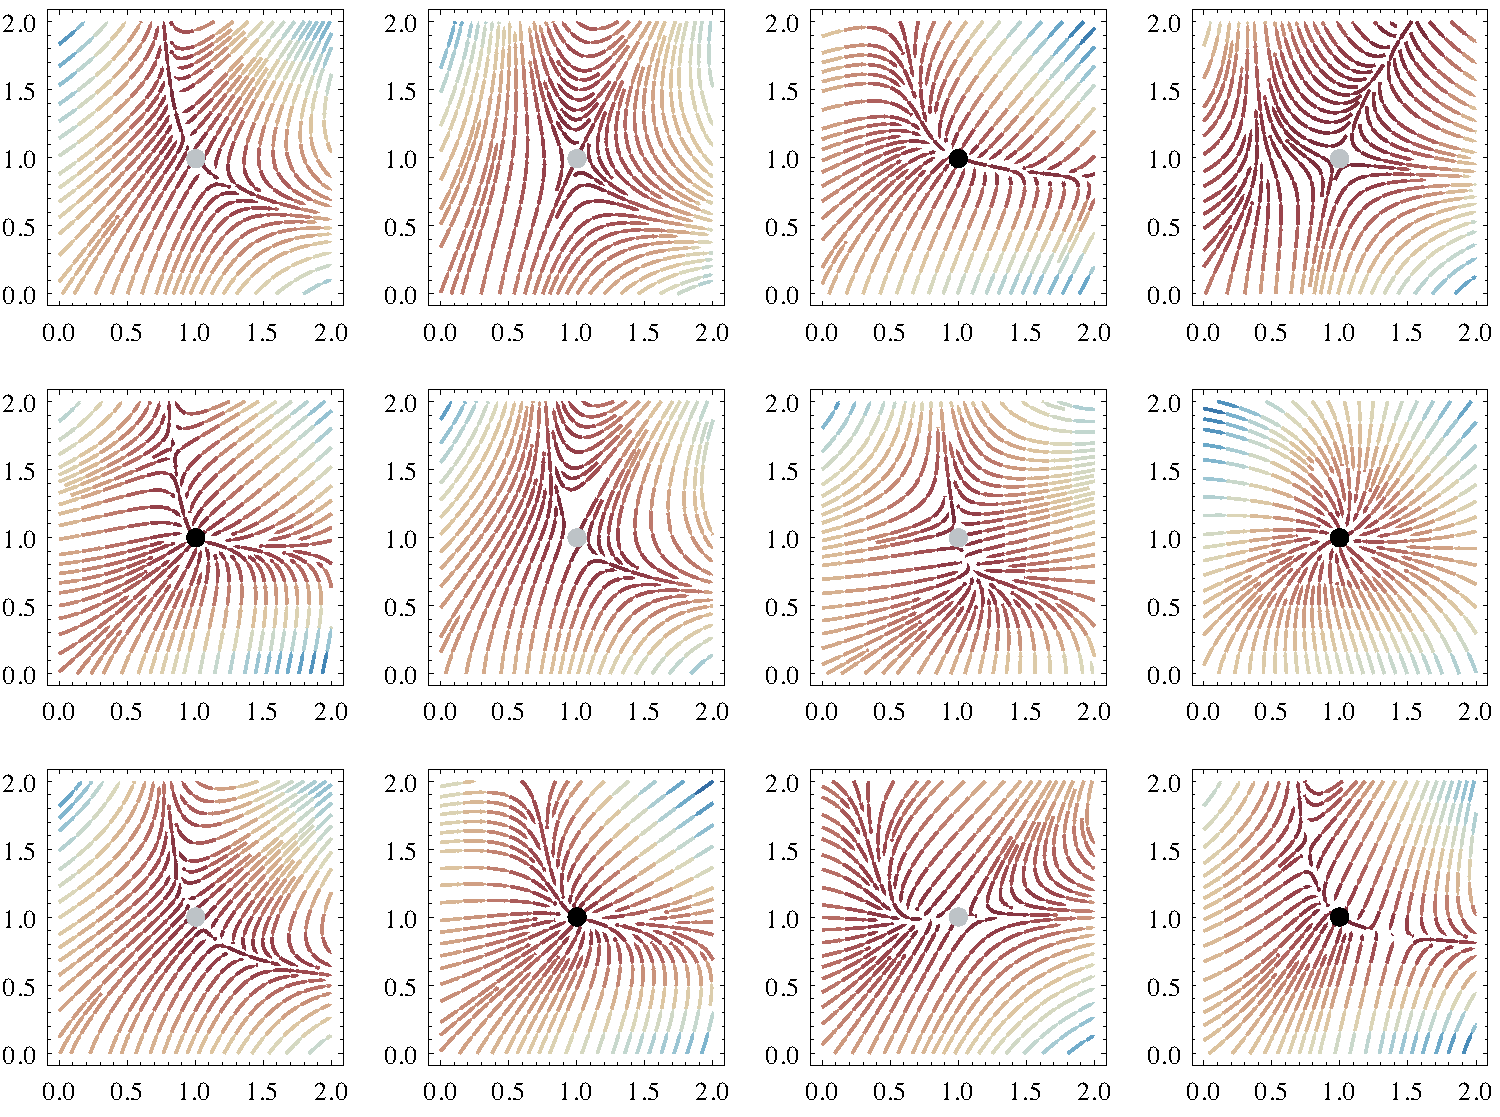
\includegraphics[width=0.9\columnwidth]{fig/jacobianvectorfields.pdf}
\caption{{\bf Vector fields resulting from the random sampling of two component systems.} System parameters of \ref{eq:arbitraryjacobianreactionnetwork} are rescaled to ensure the fixed point is located at $(1,1)$. The color of the dot located at the fixed point indicates whether it is stable (black) or unstable (gray).}
\label{fig:jacobianvectorfields}
\end{figure}

\pagebreak

\begin{figure}[!ht]
\centering
\noindent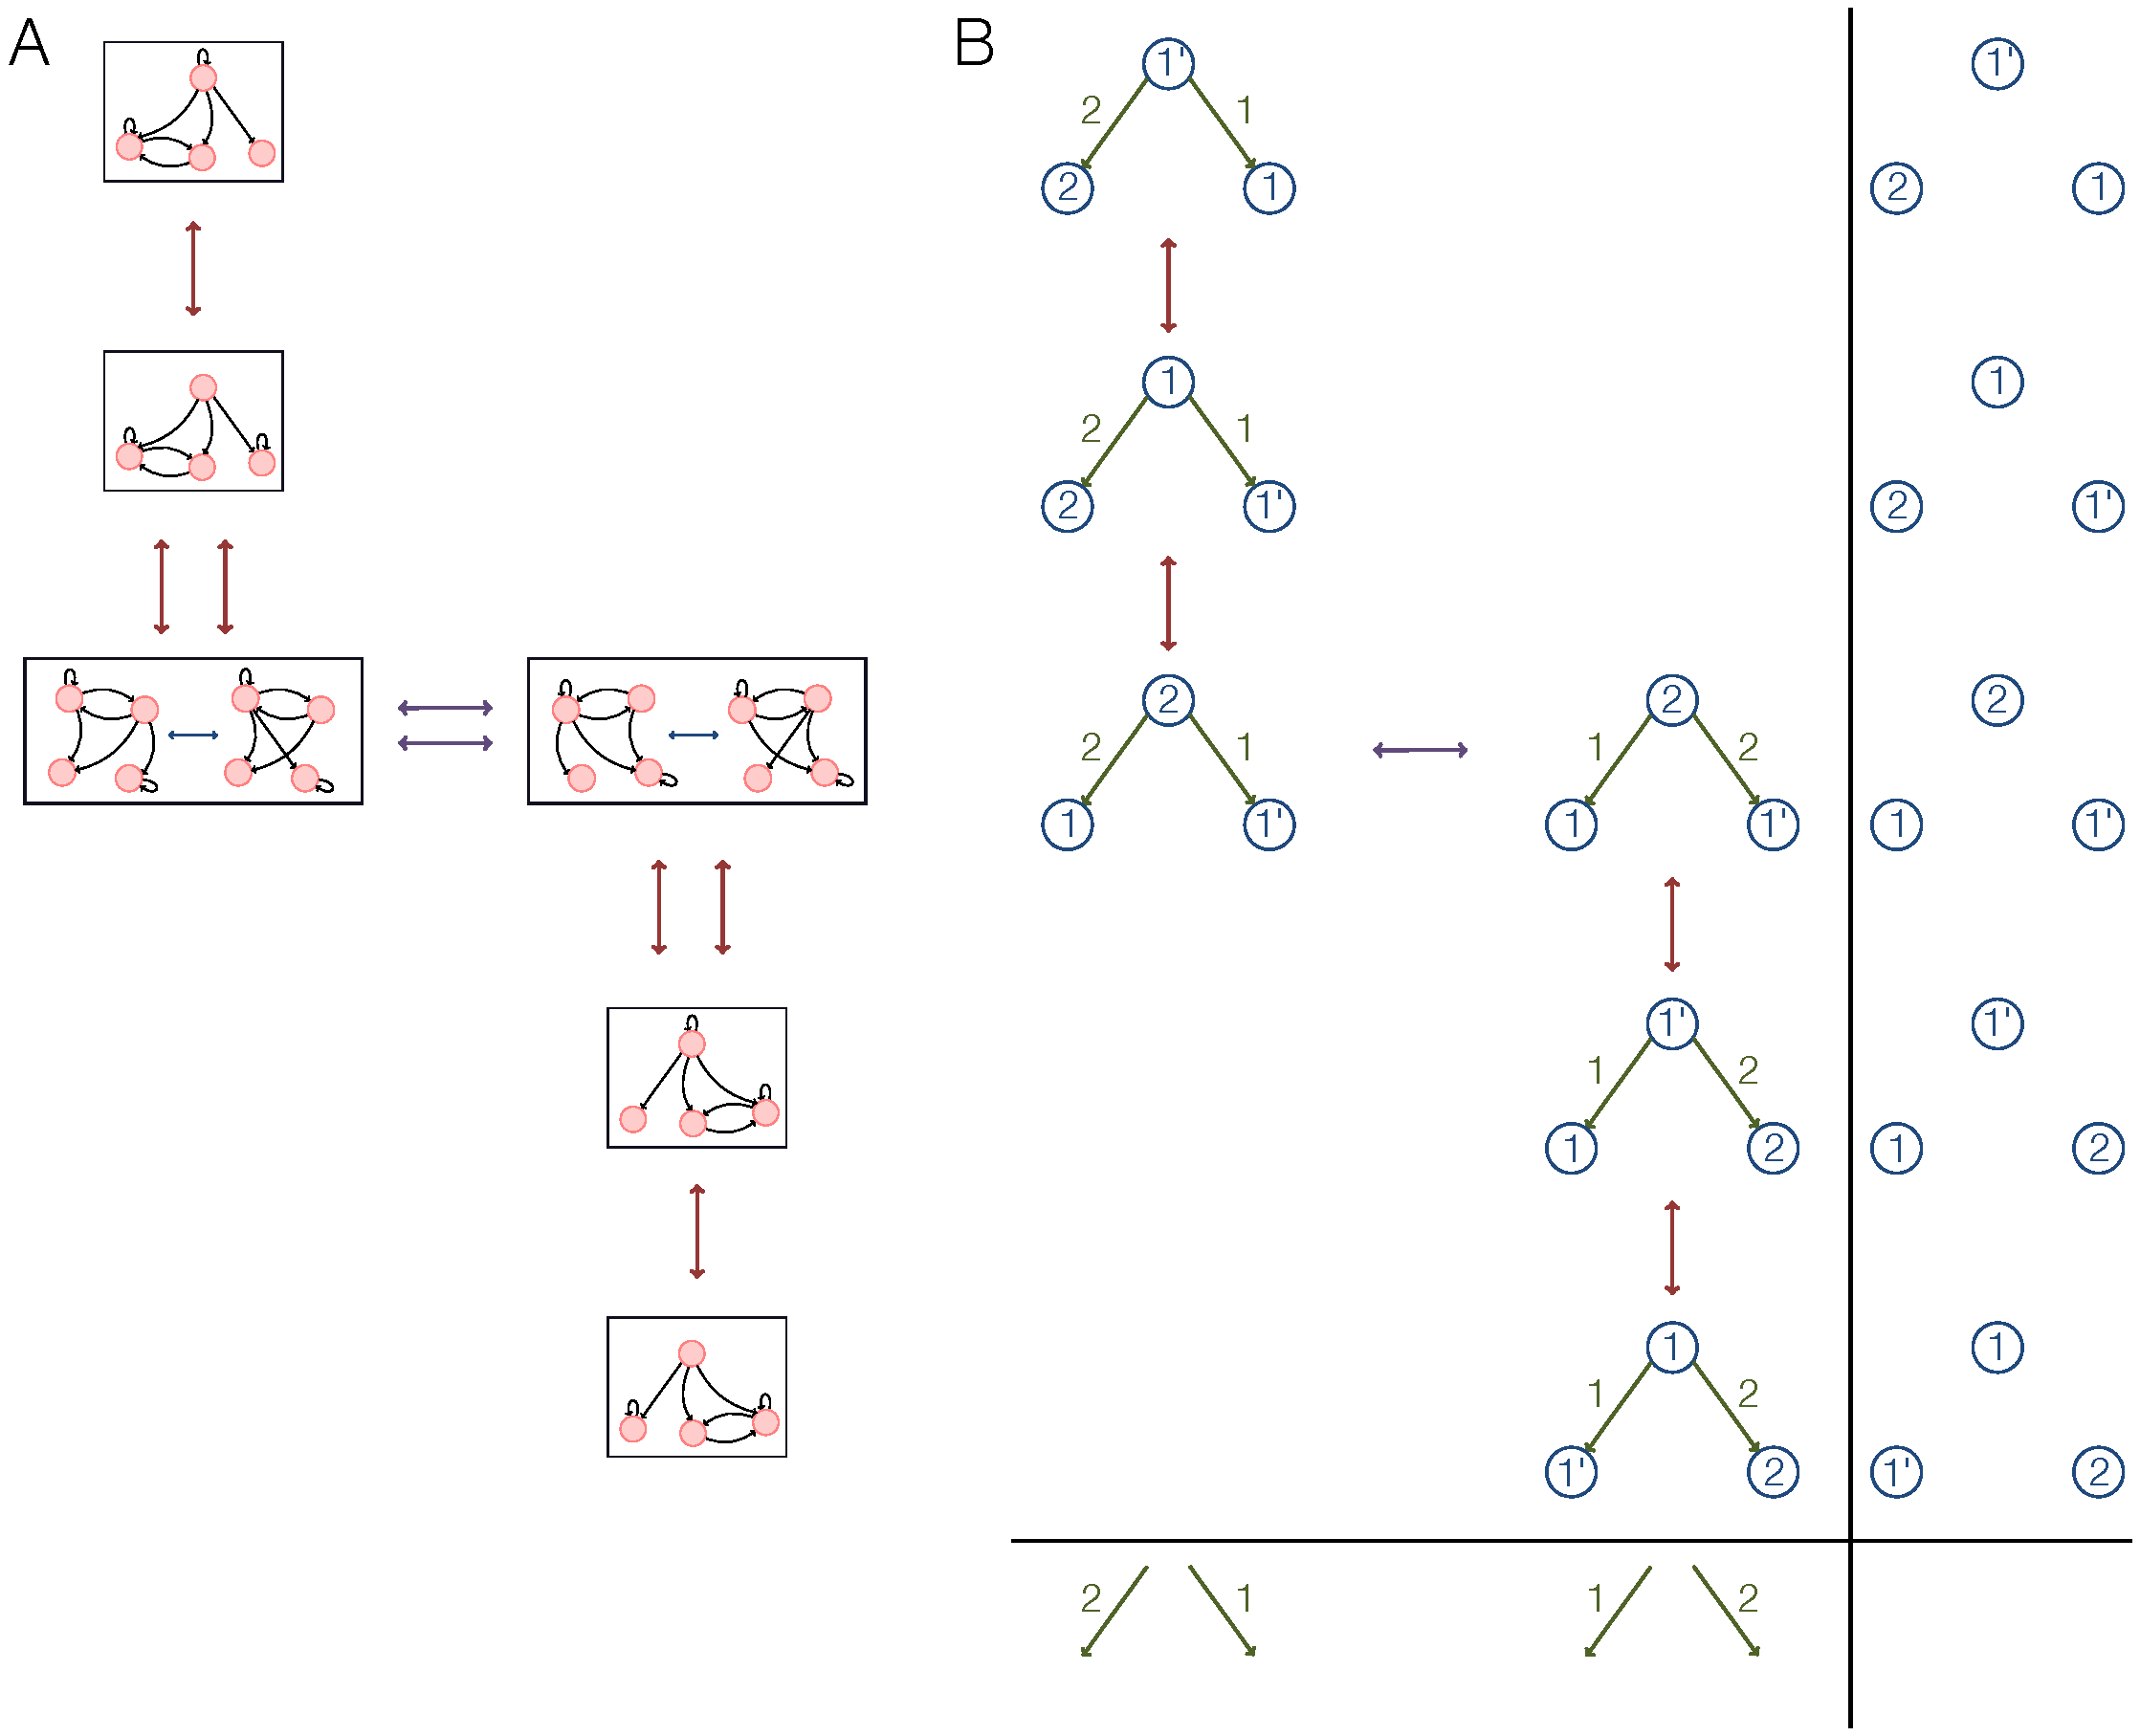
\includegraphics[width=0.9\columnwidth]{fig/robustnesssymmetries.pdf}
\caption{{\bf Example symmetries of robustness.} In this example, the connected component sizes are fixed at $\{2,1,1\}$ with a total of $3$ links between them. Red arrows correspond to transformations like \reffighiertransformations a where SCCs are swapped whereas purple arrows correspond to transformations like \reffighiertransformations b where links are moved between nodes within a SCC. (A) shows all underlying graphs while (B) shows the number of nodes in each SCC and the number of links between the SCCs.}
\label{fig:robustnesssymmetries}
\end{figure}

\pagebreak

\begin{figure}[!ht]
\centering
\noindent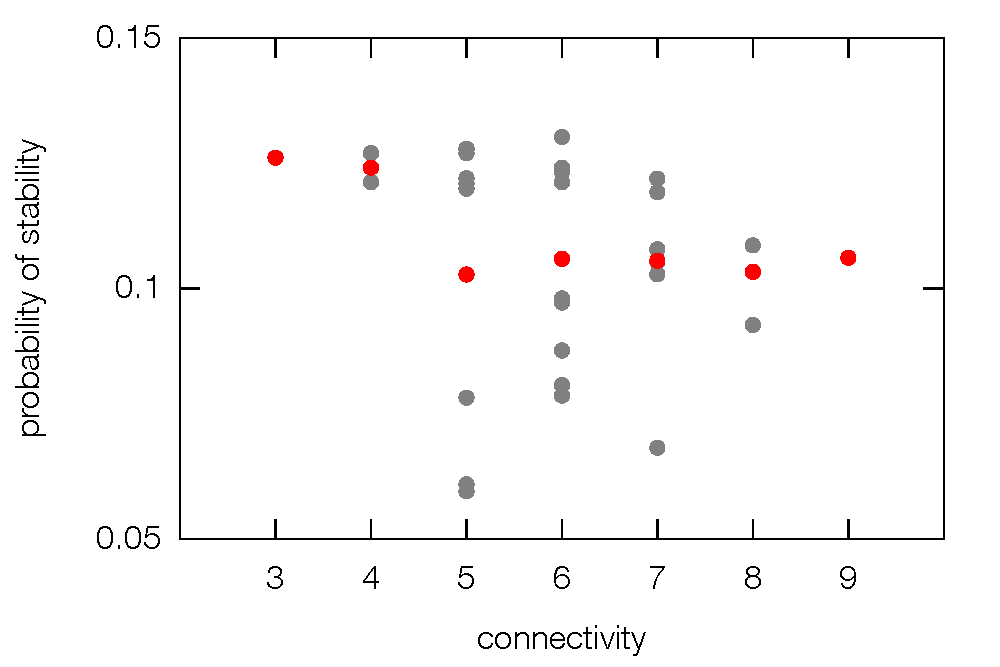
\includegraphics[width=0.6\columnwidth]{fig/apstab3x3.pdf}
\caption{{\bf System stability as a function of connectivity.} The probability of stability is plotted versus connectivity for all three component systems. We note that, in contrast to robustness, the stability ranges over less than 10\% of the possible dynamic range and demonstrates no obvious significant correlation with connectivity. The red points represent the average of system stability at each connectivity.}
\label{fig:apstab3x3}
\end{figure}

\pagebreak
\FloatBarrier

\begin{figure}[!ht]
\centering
\noindent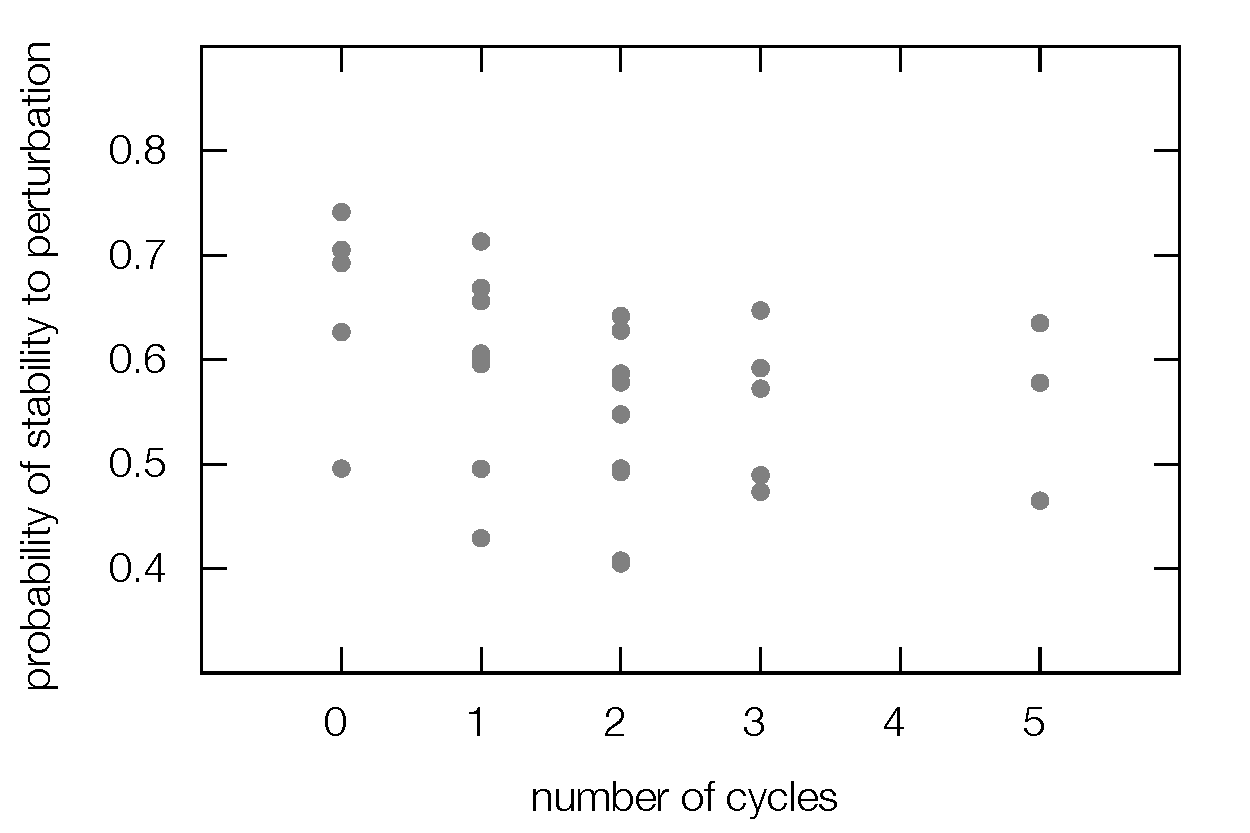
\includegraphics[width=0.6\columnwidth]{fig/cycle3x3.pdf}
\caption{{\bf Dynamical robustness as a function of cycle number.} Note that number of cycles alone does not classify networks according to their dynamical robustness.}
\label{fig:cycle3x3}
\end{figure}

% \begin{figure}[!ht]
% \centering
% \noindent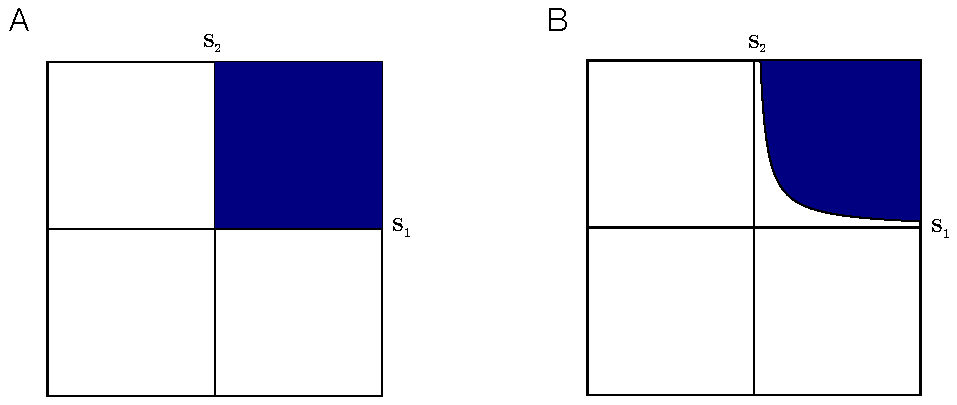
\includegraphics[width=0.7\columnwidth]{fig/region2and3.pdf}
% \caption{{\bf Stability conditions on coefficients of the characteristic polynomial for two and three variable systems.} The regions correspond to all possible relationships between the invariants determined by the characteristic polynomial.}
% \label{fig:region2and3}
% \end{figure}

% \pagebreak

% \begin{figure}[!ht]
% \centering
% \noindent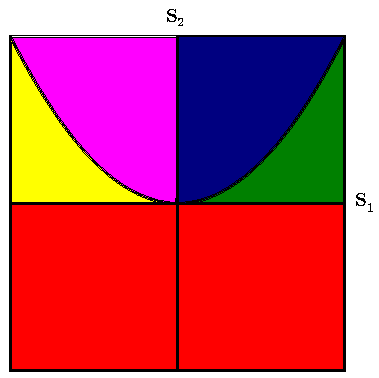
\includegraphics[width=0.5\columnwidth]{fig/region2x2.pdf}
% \caption{{\bf Stability conditions on coefficients of the characteristic polynomial for two variable systems.} The regions correspond to all possible relationships between the invariants determined by the characteristic polynomial. Colors correspond to the regions given in the main text Green: $R_{2000}$, Red: $R_{1100}$, Yellow: $R_{0200}$, Magenta: $R_{0002}$, Blue: $R_{0020}$.}
% \label{fig:region2x2}
% \end{figure}

% \pagebreak

% \begin{figure}[!ht]
% \centering
% \noindent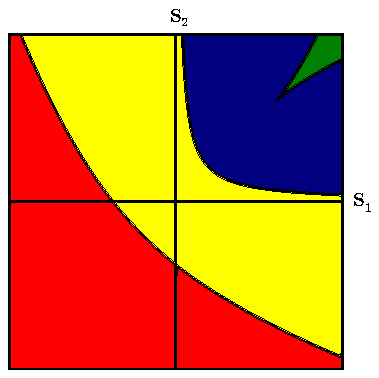
\includegraphics[width=0.5\columnwidth]{fig/region3x3.pdf}
% \caption{{\bf Stability conditions on coefficients of the characteristic polynomial for three variable systems.} Colors correspond to the following regions Green: $R_{3000}$, Red: $R_{1200}$, Yellow: $R_{1002}$, Blue: $R_{1020}$. This is the plane $s_3=1$.}
% \label{fig:region3x3}
% \end{figure}


\end{document}

%------------------------------------------------------------------------------
% End of journal.tex
%------------------------------------------------------------------------------
